\section{Problem Definition}\label{sec:model}

As described informally in the introduction, the model combines three components: (1) the substrate network (the servers
and the connecting physical network),
(2) the input which needs to be processed (divided into data chunks), and
(3) the virtual network (the virtual machines and the logical network connecting the machines to each other
as well as to the chunks).

\textbf{\emph{The Substrate Network.}} The substrate network (also known as the \emph{host graph}) represents the physical resources:
a set~$S$ of~$n_S=|S|$ servers interconnected by a network consisting of a set~$R$ of routers (or switches)
and a set~$E$ of (symmetric) links; we will often refer to the elements in~$S\cup R$
as the \emph{vertices}. We will assume that the inter-connecting network forms an (arbitrary, not necessarily balanced
or regular) tree,
where the servers are located at the tree leaves.
Each server~$s\in S$ can host a certain number
of virtual machines (available server capacity~$\capacity(s)$), and each link~$e\in E$ has a certain bandwidth
capacity~$\capacity(e)$.

\textbf{\emph{The Input Data.}} The to be processed data constitutes the input to the batch-processing application.
The data is stored in a distributed manner; this spatial distribution is given and not subject to optimization.
The input data consists of~$\tau$ different \emph{chunk types}~$\{\achunk_1, \ldots, \achunk_{\ChunkType}\}$,
where each chunk type~$\achunk_i$ can have~$r_i\geq 1$ instances (or replicas)~$\{\achunk_{i}^{(1)},\ldots, \achunk_{i}^{(r_i)}\}$,
 stored at different servers. A single server may host multiple chunks.
It is sufficient to process one replica, and we will sometimes refer to this
replica as the \emph{active} (or selected) replica.

\textbf{\emph{The Virtual Network.}} The virtual network consists of a set~$\VirtualNodes$ of~$n_V=|\VirtualNodes|$ virtual machines,
henceforth often simply called \emph{nodes}.
Each node~$v \in \VirtualNodes$ can be placed (or, synonymously, \emph{embedded}) on a server; this placement can be subject
to optimization.

Depending on the available capacity~$\capacity(s)$ of server~$s$, multiple nodes may be hosted on~$s$.
We will denote the server~$s$ hosting node~$v$ by~$\pi(v)=s$.
Since these nodes process the input data, they need to be assigned and connected to the
chunks. Concretely, for each chunk type~$\achunk_i$, exactly one
replica~$\achunk_{i}^{(j)}$ must be processed by exactly one node~$v$;
which replica~$\achunk_{i}^{(k)}$ is chosen is subject to optimization, and
we will denote by~$\mu$ the assignment of nodes to chunks.

In order to ensure a predictable application performance, both the connection to the chunks
as well as the interconnection between the nodes may have to ensure certain
minimal bandwidth guarantees; we will refer to the first type of virtual network as the \emph{(chunk) access
network}, and to the second type of virtual network as the \emph{(node) inter-connect}; the latter
is modeled as a complete network (a \emph{clique}). Concretely, we assume that an  active chunk
is connected to its node at a minimal (guaranteed) bandwidth~$\CostTrans$, and a node is connected to any other node
at minimal (guaranteed) bandwidth~$\CostCom$.
Figure~\ref{fig:overview} gives an overview of our model.

\begin{figure}[t]
\centering
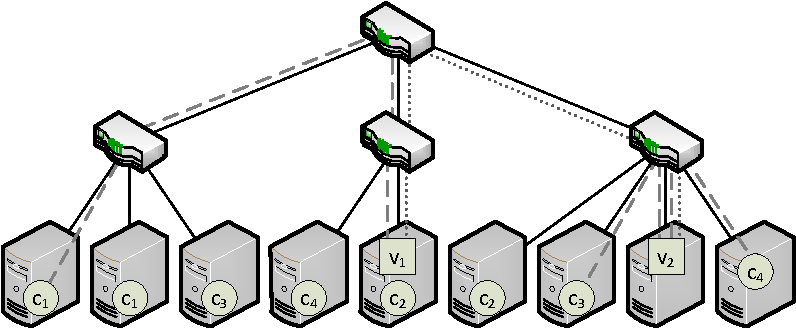
\includegraphics[width=0.79\columnwidth]{figs/static-mapping/data_locality_no_legend.pdf}
\caption{Overview: a 9-server datacenter storing~$\tau=4$ different chunk
types~$\{c_1,\ldots,c_4\}$ (depicted as \emph{circles}). The chunk replicas need to be selected and assigned to the two
 virtual machines~$v_1$ and~$v_2$; the virtual machines are depicted as \emph{squares}, and
 the network connecting them to chunks (at bandwidth~$\CostTrans$) is \emph{dashed}. In addition, the virtual machines are inter-connected among
 each other at bandwidth~$\CostCom$ (\emph{dotted}). The objective of the embedding algorithm is to minimize the overall bandwidth allocation
 (sum of \emph{dashed} and \emph{dotted} lines).}\label{fig:overview}
\vspace{-1em}
\end{figure}


\subsection{Optimization Objective}

Our goal is to develop algorithms which 
accept and embed a request
whenever this is possible, and minimize the \emph{resource footprint}: the amount of resources which have to be dedicated to a request, in order to realize its guarantees.
Essentially, the footprint captures the overall resource allocation, and is the most common objective function considered in the literature (a.k.a.~as the min-sum objective guarantee)
\cite{fischer-survey}.

Formally, let~$\dist(v,\achunk)$ denote the distance (in the underlying physical network~$\Tree$) between a node~$v$ and
its assigned (active) chunk replica~$\achunk$, and let~$\dist(v_1,v_2)$ denote the distance between the two nodes~$v_1$ and~$v_2$.
We define the \emph{footprint}~$\Cost(v)$ of a node~$v$ as follows:
$$
\Cost(v) = \sum_{\achunk\in \mu(v)} \CostTrans \cdot \dist(v,\achunk) \underbrace{+ \frac{1}{2} \cdot \sum_{v' \in \VirtualNodes\setminus\{v\}} \CostCom \cdot \dist(v,v')}_{\text{only for inter-connect}},
$$
 where~$\mu(v)$ is the set of chunks assigned to~$v$. Our goal is to minimize the overall footprint
$\Cost=\sum_{v\in V} \Cost(v)$.

\subsection{Problem Decomposition}

In order to chart the landscape of the computational tractability and intractability of different
problem variants, we decompose our problem into its fundamental aspects, namely replica selection
($\RS$), multiple chunk assignment ($\MA$), flexible node placement ($\FP$), node interconnect ($\CC$),
and bandwidth constraints ($\BW$), as described in the following. 
In this chapter, we will consider all possible 32 problem variants, where each of these five aspects
can either be enabled or disabled. 

\textbf{\emph{Replica Selection ($\RS$).}} The first fundamental problem is replica selection:
if the input data is stored redundantly, the algorithm has the freedom to choose a replica
for each chunk type, and assign it to a virtual machine (i.e., \emph{node}).
In the following, we will refer to a scenario
with redundant chunks by~$\RS$; in the~$\RS$-only scenario, the number of chunk types
is equal to the number of nodes. Otherwise, we will add the~$+\MA$ property discussed next.

\textbf{\emph{Multiple Assignment ($\MA$).}}
If the number of chunk types~$\tau$ is larger than the number of nodes,
each node needs to be assigned multiple chunks. We will refer to such a scenario by~$\MA$. 
Since all nodes are identical and no additional information regarding the chunks is available at request time, we assume that each node will process an identical integer number of chunks~$\MaFactor = \tau / n_V$. 


\textbf{\emph{Flexible Placement ($\FP$).}} %The third fundamental degree of freedom, besides replica selection and assignment,
While the nodes are placed a priori in some cases, the node placement (or
synonymously: \emph{embedding}) of nodes on physical servers can also be
subject to optimization. We will refer to this degree of freedom by FP.

\textbf{\emph{Node Interconnect ($\CC$).}} We distinguish between scenarios
where bandwidth needs to be reserved
both from each node to its assigned chunks as well as to the other nodes
(i.e.,~$\CostTrans>0$ and~$\CostCom>0$), and
 scenarios where only the (chunk) access network requires bandwidth reservation (i.e.,~$\CostTrans>0$ and~$\CostCom=0$).
 We will refer to the former scenario
where bandwidth needs to be reserved also for the inter-connect, by~$\CC$. 
The node interconnect is modelled as a complete graph, to account for the all to all communication patterns of batch processing applications such as MapReduce.


\textbf{\emph{Bandwidth Capacities ($\BW$).}}
We distinguish between an uncapacitated and a capacitated scenario where the links
of the substrate network come with bandwidth
constraints, and will refer to the bandwidth-constrained version by~$\BW$; the capacity of servers
(the number of nodes which can be hosted concurrently) is always limited.
Note that capacity constraints introduce infeasible problem instances, where it is impossible to
allocate sufficient resources to satisfy an embedding request.

\section{Polynomial-Time Algorithms}\label{sec:poly}


Despite the various degrees of freedom in terms of embedding and replica selection,
we can solve many problem variants efficiently.
 This section introduces three general techniques,
 which can roughly be categorized into
 \emph{flow} (Section~\ref{ssec:flow}), \emph{matching} (Section~\ref{ssec:match}) and \emph{dynamic programming}
 (Section~\ref{ssec:dyn}) approaches.
First, let us make a simplifying observation:
\begin{obs}\label{obs:nofp}
In problems without flexible placement ($\FP$),
the bandwidth required
for the inter-connect network ($\CC$) can be allocated \emph{upfront}, 
as it
does not depend on the replica
selection and assignment.
Accordingly, we can reduce problem variant~$\RS+\MA+\CC +\BW$ (as well as all its subproblems)
to~$\RS+\MA+\BW$ (resp.~its subproblems).
\end{obs}

\subsection{Flow Algorithms}\label{ssec:flow}


\begin{figure}[t]
\centering
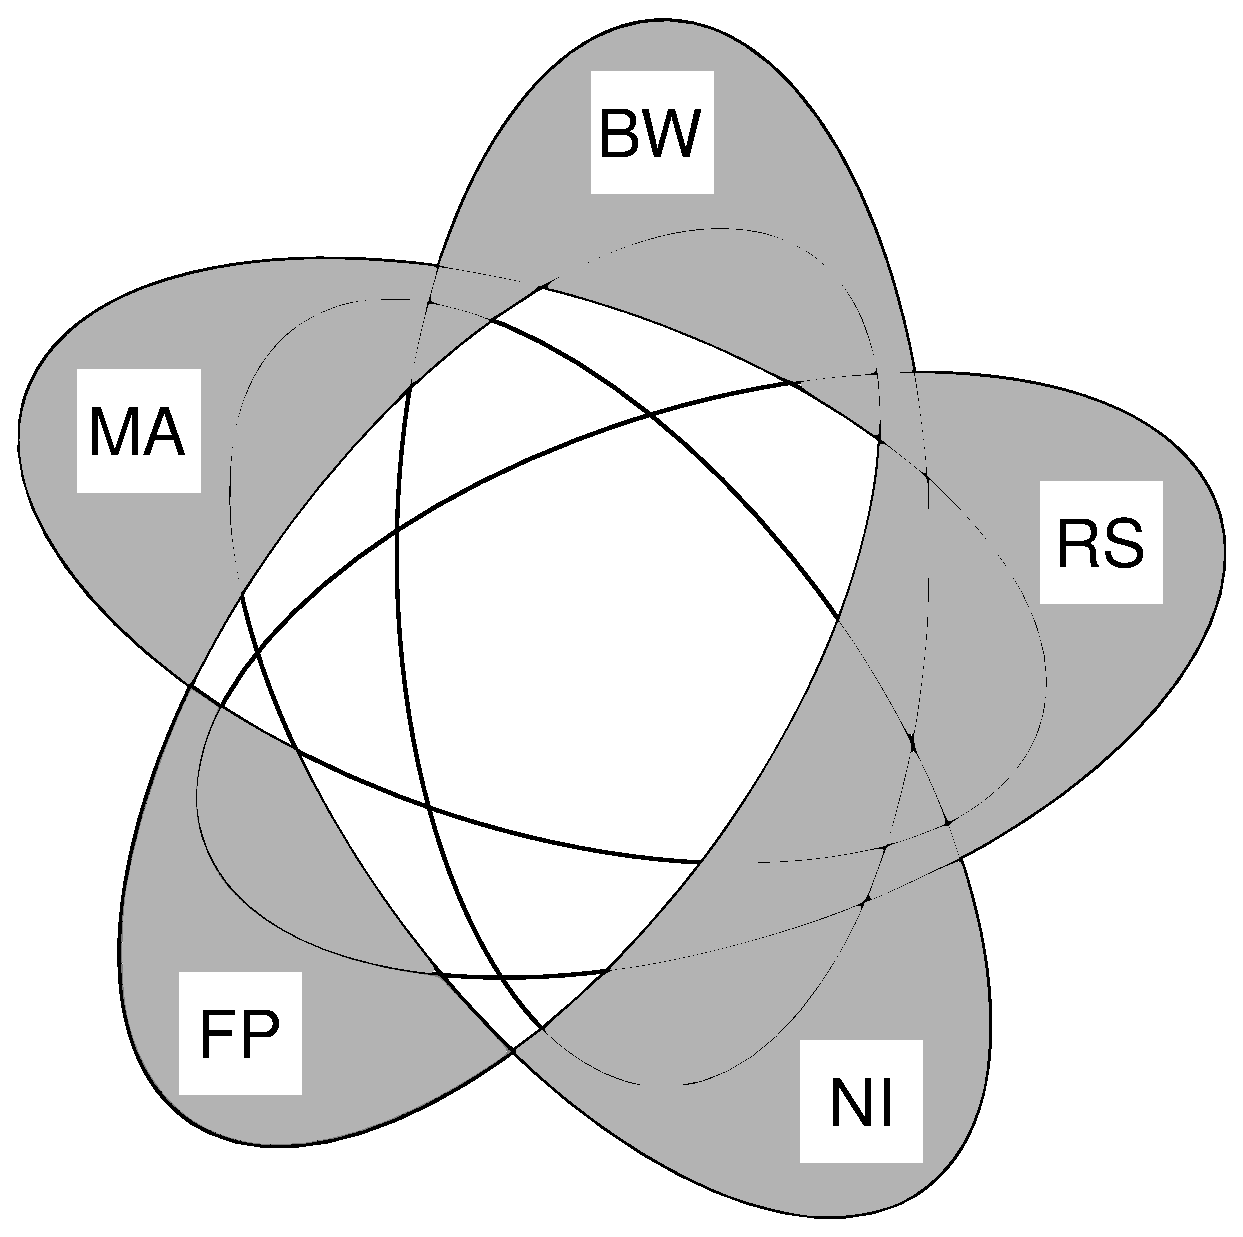
\includegraphics[width=0.49\columnwidth]{figs/static-mapping/venn_flow.pdf}
\caption{Variants solved by flow approach.}
\vspace{-1em}
\label{fig:venn_flow}
\end{figure}


We first present an algorithm to solve the~$\RS+\MA+\CC+\BW$ problem.
Recall that in this problem variant,
we are given a set of redundant chunks ($\RS$) and a set of
nodes
(the \emph{nodes})
at fixed locations (no~$\FP$). The number of chunk types is larger than the number
of nodes ($\MA$), and each node needs to be connected
to its selected chunks as well as to other nodes ($\CC$), while respecting
capacity constraints ($\BW$).
Our goal is to minimize the resource footprint~$\Cost$, consisting
of the bandwidth reservations in the (chunk) access network and the (node)
inter-connect.
As we will see in the following, we can use a flow approach to solve this
problem variant.




\textbf{Construction of Artificial Graph.}
In order to solve the~$\RS+\MA+\CC+\BW$ problem,
we first remove the~$\CC$ property using Observation~\ref{obs:nofp}.
We then construct
an artificial graph~$\Tree^*$, extending the substrate network~$\Tree$ and
normalizing bandwidth capacities, as follows. For~$\Tree^*$,
we normalize the bandwidth of~$\Tree$ to integer multiples of~$\CostTrans$,
i.e., for each link~$e\in E(\Tree)$, we set its new
capacity in~$\Tree^*$ to~$\lfloor\capacity(e)/\CostTrans\rfloor$.
After this normalization, we extend the topology~$\Tree$ by
introducing an artificial vertex for each chunk type. These artificial
vertices are connected to each leaf (i.e., server) in~$\Tree$ where a replica
 of the respective chunk type is located,
connecting the replica of the respective chunk type by a link of capacity~$1$. In
addition, we create a
\emph{super-source}~$\Source$, and connect it to each of the artificial chunk
type vertices (with a link of capacity 1). Moreover, we create an artificial \emph{super-sink}~$\Sink$ and
connect it to every leaf containing at least one node; the link capacity represents
the number of nodes~$x$ hosted on this server, times the multi-assignment factor
$\MaFactor$.
We additionally assign the following costs to edges of~$\Tree^*$:
every edge of the original substrate network costs one unit, and all other artificial edges
cost nothing.

A solution to the~$\RS+\MA+\BW$ problem can now be computed
from a solution to the \emph{Min-Cost-Max-Flow} problem between super-source
$\Source$ and
super-sink~$\Sink$ on the artificial graph~$\Tree^*$.

\textbf{Example.} Figure~\ref{fig:flow_construction} shows an example of the extended substrate
network~$\Tree^*$: The sink~$\Sink$ is connected to the two leaves, which host the
nodes. The artificial nodes are depicted below the leaves, are labeled with
their respective chunk types (e.g.,~$\achunk_1$), and are connected to the source
$\Source$ as well as to the leaves which contain replicas of their chunk type.
The
maximum flow with minimal costs is indicated by the dashed lines: each line
represents one unit of flow. The dotted lines indicate links which have reduced
capacity due to~$\CC$.

\begin{figure}
\centering
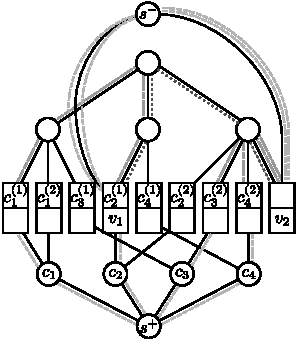
\includegraphics[width=0.45\columnwidth]{figs/static-mapping/flow_ma_cv}
\caption{Example of flow construction: Problem instance with two nodes, four chunk
types, and two replicas per type. The min-cost-max-flow
is indicated by the dashed lines: each line represents one unit of flow.
}
\vspace{-1em}
\label{fig:flow_construction}
\end{figure}

\textbf{Algorithm.}
Our algorithm to solve~$\RS+\MA+\CC+\BW$ consists of three parts:
\emph{First}, we construct the normalized and extended graph~$\Tree^*$
described above and compute
a min-cost-max-flow solution, e.g.,
using~\cite{mincostmaxflow-1,mincostmaxflow-2}.
\emph{Second}, we have to \emph{round} the resulting, possibly fractional flow, to
integer values. Due to the \emph{integrality theorem}~\cite{flow-book},
there always exists an optimal integer solution on graphs with integer capacities.
However, while algorithms like the successive shortest path algorithm~\cite{successive_shortest_path_complexity}
directly give us such an integral solution (in polynomial time), the fastest min-cost-max-flow algorithms (e.g., based on double-scaling
methods~\cite{mincostmaxflow-1} or minimum mean-cost cycle
algorithms~\cite{mincostmaxflow-2}, may yield fractional solutions
which need to be rounded to integral solutions (of the same cost).
In order to compute integral solutions, we proceed as follows: we iteratively
pick an arbitrary (loop-free) path
currently having a fractional allocation of value~$f$ ($f>0$), and distribute its flow~$f$
among all other fractional paths of the same length; due to the optimality of the fractional solution
and due to the integrality theorem, such paths must always exist. After distributing this flow,
the total allocation on this path will be 0, and we have increased the number of
integer paths by at least one. We proceed until we constructed the perfect
matching.
\emph{Third}, given an integer min-cost-max-flow solution, we need to decompose
the integer flow into the paths
representing matched chunk-node pairs:
The assignment can be obtained by decomposing the flow allocated in the
original substrate network. In order to identify a matched chunk-node pair,
we take an arbitrary (loop-free) path~$p$ carrying a flow of value ~$\geq 1$ from~$\Source$ to~$\Sink$:
the first hop represents the chosen chunk type, the second hop the chosen
replica, and the last but one hop represents the server: we will assign
the replica to an arbitrary unused node on this server.
Having found this pair, we reduce the flow
along the path~$p$ by one unit.
We continue the pairing process until every chunk type is assigned.

\textbf{Analysis.}
The correctness of our approach follows from our construction
of~$\Tree^*$, using integer capacities (in our case~$\lfloor\capacity(e)/\CostTrans\rfloor$),
and the fact that cost optimal integral solutions always exist~\cite{flow-book}.
The runtime of our algorithm consists of four parts: construction of~$\Tree^*$,
computation of the min-cost-max-flow, flow rounding, and decomposition. The
dominant term in the asymptotic runtime is the flow computation.
Using the state-of-the-art min-cost-max-flow
algorithms~\cite{mincostmaxflow-1,mincostmaxflow-2}
we get a runtime of~$\mathcal{O}(n_S^2 \cdot \log\log \min \{U,\tau\})$
where~$U$ is the maximal link capacity; note that in networks with high capacity
and uncapacitated networks, we can simply set~$U=\tau$.


\subsection{Matching Algorithms}\label{ssec:match}


\begin{figure}[t]
\centering
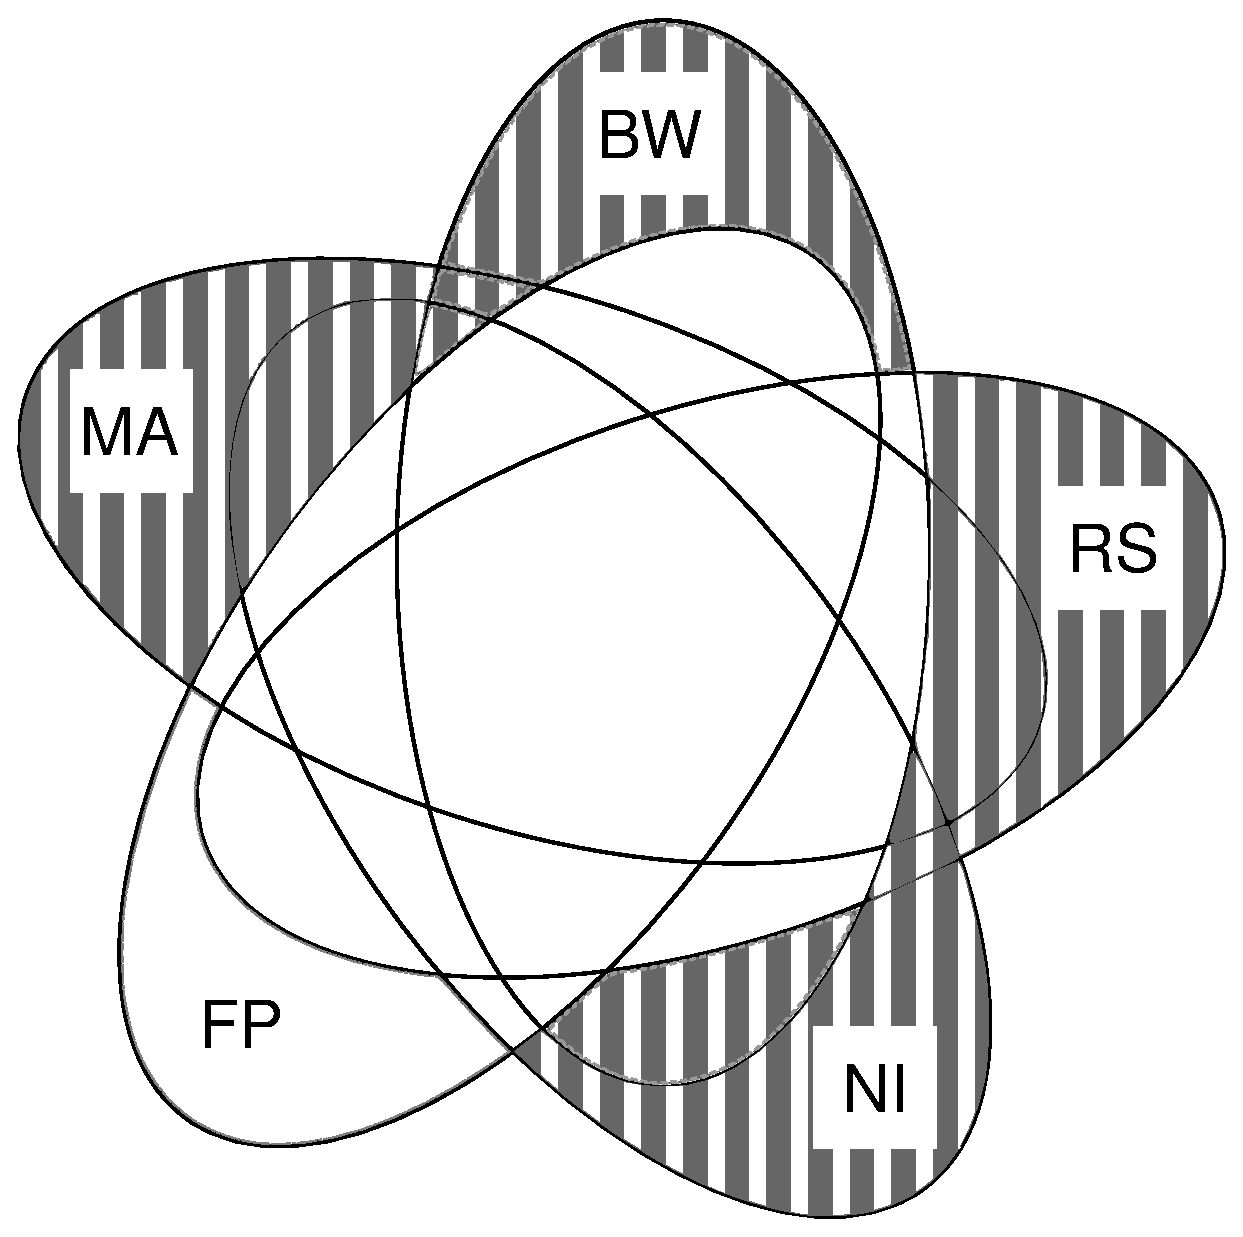
\includegraphics[width=0.49\columnwidth]{figs/static-mapping/venn_matching.pdf}
\caption{Variants solved by matching approaches.}
\vspace{-1em}
\label{fig:venn_match}
\end{figure}
This section presents faster algorithms to solve 
the two problem variants
$\RS+\MA+\CC$ and~$\MA+\CC+\BW$ which can also be solved with the flow approach
introduced above.
In general, we refer to the algorithms presented in this section
as matching approaches.


\subsubsection{$\RS+\MA+\CC$}

Let us first consider the~$\RS+\MA+\CC$ variant.
Recall that in this problem,
we are given a set of redundant chunks ($\RS$) and a set of nodes
at fixed locations. The number of chunk types is larger than the number
of nodes ($\MA$), and each node needs to be connected
to its chunks as well as to other nodes ($\CC$).
Our goal is to minimize the resource footprint~$\Cost$, consisting
of the bandwidth reservations in the access network and the inter-connect.

\textbf{Algorithm.} Due to Observation~\ref{obs:nofp},~$\RS+\MA+\CC$ degenerates to~$\RS+\MA$.
In order to solve the~$\RS+\MA$ problem variant,
we construct a bipartite
graph between the set
$\VirtualNodes$ of nodes and
the set of chunks.
Concretely, we clone each node~$\MaFactor$ times,
as each node needs to process
$\MaFactor$ chunk types, and we collect all copies of a given chunk type in a
single %$\ChunkType$
``super-node''. We connect each node to all chunk types using the
\emph{lowest hop count} to one of the copies as the cost metric (the link weight).
On the resulting bipartite graph, we can now compute a \emph{Minimum Weight
Perfect
Matching}~\cite{gabow_scaling_algorithm}:
the resulting matching describes the optimal assignment of chunks to nodes.
\begin{figure}
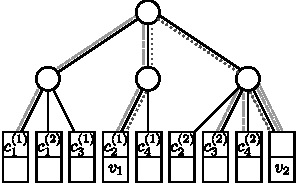
\includegraphics[width = 0.49\columnwidth]{figs/static-mapping/model_ma_r_cv_boxes}
\hfill
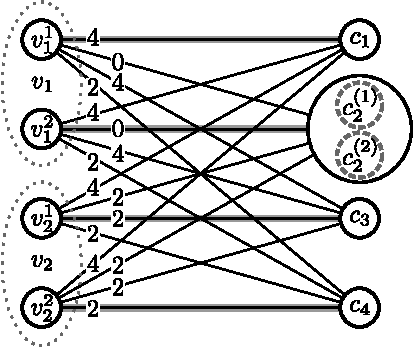
\includegraphics[width =0.49\columnwidth]{figs/static-mapping/matching}
\caption{The~$\RS+\MA$ problem on the \emph{left} is converted into a
matching problem on the \emph{right}. Since each node has to process two
chunks, the
nodes are replicated in the matching representation. The two replicas of each
chunk type are represented by a single node, and all edges connecting to this
node have a weight according to the shorter distance to one of the replicas.
This is visualized for~$\achunk_2$.}
\label{fig:matching}
\end{figure}

\textbf{Example.} Before analyzing our algorithm, let us consider a small example.
Figure~\ref{fig:matching} illustrates
an instance where two nodes are
cloned into~$\MaFactor = 2$ nodes each,
resulting in a total of four nodes in
the matching problem representation.
The two replicas of each chunk type are
aggregated into a single chunk type vertex~$\achunk_j$  in the matching problem;
this gives a total of four chunk type vertices in the matching graph. The costs
on the links between all clones of a specific vertex and a chunk type are set to
the minimum distance. We can observe this for instance at the edges connecting
the two clones of~$\VirtualNode_1$ to~$\achunk_2$: both weights are 0.

\textbf{Analysis.}
The correctness of our algorithm follows from the construction and the optimal
solution of the minimum matching.
The runtime consists of two parts: the construction of the matching graph and
the actual matching computation. The constructed graph consists of
$\MaFactor \cdot n_V \cdot \ChunkType$
many edges,
and for each edge we need to compute its cost, i.e., the shortest distance
which in a tree can be computed in time~$n_S$; thus, the overall construction time
is
$\mathcal{O}(n_S \cdot \tau^2)$.
The state of the art algorithm to compute matchings are based on scaling techniques~\cite{scale-match}.
The runtime translates to
$\mathcal{O}(\tau^{5/2}\cdot \log(\tau\cdot n_S))$; recall that~$\tau = \MaFactor\cdot n_V$.




\subsubsection{Faster~$\MA+\CC$ and~$\MA+\CC+\BW$}

We now show that we can solve~$\MA+\CC$ even faster, by exploiting
locality. Moreover, we will show that we can
even solve
$\MA+\CC+\BW$ problem variants by simply
verifying feasibility.
In the following, due to Observation~\ref{obs:nofp}, we can focus on
the~$\MA$ resp.~$\MA+\BW$ problem.

We first introduce the following definition.
\begin{defn}[Local Assignment (LA)]\label{def:loc}
We define an assignment~$\VmChunkAssignment$ to
be \emph{local in a specific subtree~$\Tree'$}, iff~$\VmChunkAssignment$
assigns the maximum number of chunks in the
subtree to nodes in the same subtree.
We define~$\VmChunkAssignment$ to be \emph{local} when
it is local with respect to all possible subtrees of the substrate network.
\end{defn}

\begin{figure}
\center
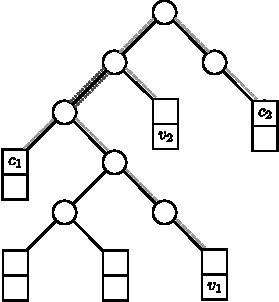
\includegraphics[width = 0.45\columnwidth]{figs/static-mapping/unbalanced_tree}
\caption{Illustration of local assignment: The dashed lines indicate bandwidth allocations, which occur
independently of the chosen assignment. The dotted lines indicate bandwidth
allocation which occur only if~$c_2$ is assigned to~$v_1$.}
\label{fig:unbalanced_tree}
\end{figure}

\textbf{Example.}
Figure \ref{fig:unbalanced_tree} illustrates the concept of local assignment:
The closest chunk to~$v_2$ is~$c_1$, and the closest node to~$c_1$ is~$v_2$.
However, a subtree~$T'$ exists such that~$v_1 \in T'$ and~$c_1
\in T'$, but~$v_2 \notin T'$. Therefore, a local assignment cannot assign~$c_1$ to~$v_2$.


We will see later that
optimal solutions to
$\MA$ have a local assignment. We exploit this in our algorithms described
in the following.

\textbf{Algorithm.} Our proposed algorithm for~$\MA$
proceeds in a bottom-up fashion, traversing the substrate network~$\Tree$
from the leaves toward the root.
For each subtree~$\Tree'$, we maintain
two sets~$S_1,S_2$ in order to match unmatched
chunks~$S_1$ in the subtree~$\Tree'$ to unmatched
nodes~$S_2$ in~$\Tree'$. Both sets are initially empty.

We first process all the leaves, in an arbitrary order; subsequently, we process arbitrary inner vertices
of~$\Tree$, whenever all their children have been processed.
We process any leaf~$\ell$
by adding any
nodes or chunks which are located on~$\ell$ to the corresponding sets~$S_1$ and~$S_2$.
A non-leaf vertex~$u$ is processed in the following way: we take the union of
the sets of~$u$'s children, i.e., the sets contain the unmatched chunks and nodes
in this subtree.
For both leaves and inner nodes, whenever
both sets are non-empty, we greedily match an arbitrary chunk in~$S_1$ with an arbitrary node in~$S_2$,
and remove them from the sets.

\textbf{Analysis.} On a given vertex~$u$, emptying one of the sets, results in a \emph{local assignment} (cf~Definition~\ref{def:loc})
in the
subtree rooted at~$u$. The bottom-up strategy ensures that this works
for every subtree in the substrate, rendering the resulting assignment
local.
The complexity of this
construction is low: For each
vertex in the substrate graph,
we build the union of the
children's sets,
and since each vertex can only be the child of one vertex,
the amortized runtime per vertex is constant; and hence the overall
runtime~$\mathcal{O}(n_S)$. The sum of all remove operations, is equal to
the number of chunk types~$\mathcal{O}(\ChunkType)$.
Hence the overall complexity of this construction amounts to
$\mathcal{O}(n_S + \ChunkType)$.

It remains to prove optimality of such local assignments.
By \emph{uplink} of a subtree with root $r$ we denote the edge from $parent(r)$ to $r$ (if it exists).
We first characterize the bandwidth allocation on uplinks of subtrees.
\begin{lemma}\label{lem:uplink-alloc}
Given an~$\MA$ problem and a subtree~$\Tree'$
containing~$x$
chunks and~$y$ nodes, the minimal bandwidth allocation of any
assignment
$\VmChunkAssignment$ on the uplink of~$\Tree'$ is~$|x-y\cdot\MaFactor|\cdot
\CostTrans$.
\label{lemma:uplink}
\end{lemma}
\begin{proof}
In case the number of chunk types equals the processing capacities of the
nodes in the given subtree,
the bandwidth allocation inflicted by the chunk access network on the uplink can
be
zero, since we can assign all chunks to nodes in the same subtree.
Otherwise, we distinguish between two cases: Recall, that in instances
without~$\RS$, all chunks have to be processed. In case
there are more chunks in the subtree, at least all of the excess chunks have to
be transferred to a different subtree, which will
inflict costs~$\CostTrans$ per excess chunk on the uplink connecting~$\Tree'$
with the
remaining parts of~$\Tree$, which will inflict costs~$\CostTrans$ per excess chunk on the uplink of root of~$\Tree'$.
 Similarly, if the processing capabilities exceed the
amount of
available chunks, excess chunks from other subtrees will have to be transferred
to
nodes in the subtree~$\Tree'$, inflicting bandwidth costs of~$\CostTrans$ each.
Hence, the minimum bandwidth allocation for the chunk access on the uplink
is the difference between the number of chunks and the processing capabilities
of the subtree~$|x-y\cdot\MaFactor|$ times the amount of bandwidth needed,
for a single transfer~$\CostTrans$.
\end{proof}


\begin{theorem}
Given an~$\MA+\CC$ problem instance, a feasible assignment~$\VmChunkAssignment$
is optimal iff it is local.
\label{thm:local_optimal}
\end{theorem}

\begin{proof}
Local assignments generate exactly the minimal allocations on all links, as
 the assignments which generate the minimal bandwidth allocations
described in
the proof of
Lemma~\ref{lemma:uplink} are local in the given subtree. Hence
each local assignment has to be optimal. A non-local assignment, has at least
one subtree, in which it is not local. This subtree will have a higher
allocation on the uplink. Since the local assignment has minimal allocations
on all other links, the non local assignment has a larger footprint.
\end{proof}



Combined with a simple postprocessing step, this approach can also solve~$\MA+\BW$. The central idea of this extension, is
that \emph{local} assignments allocate the minimal bandwidth
on each individual edge. In consequence, each bandwidth constraint
which is lower than the allocation of a local assignment on one link, renders
the problem infeasible. Hence, it is sufficient to temporarily omit the
bandwidth limitations, compute an optimal assignment for an~$\MA$ instance, and
verify that the resulting allocations do not violate any capacities. The
postprocessing step scales linearly with the number of edges in the substrate
graph.


\subsection{Dynamic Programming}\label{ssec:dyn}

We now show how to solve the~$\MA+\FP+\CC+\BW$ problem variant
in polynomial time.
Note that this problem variant requires to find a
tradeoff between the desire to place nodes as close as possible to each other
(in order to minimize communication costs), and the desire to place nodes
as close as possible to
the chunk locations.




\textbf{Example.} Figure~\ref{fig:dynamic_motivation} shows an example: one
extreme solution is to minimize the distance between chunks and nodes,
see mapping~$\NodeMapping_1$ in
Figure~\ref{fig:dynamic_motivation} \emph{(left)}: the four nodes are all
collocated with chunks, resulting in a zero-cost chunk access network. As a
result, the paths between the individual nodes are longer than in alternative
node placements: each node has a distance of two hops to one other node,
and four hops to two other nodes. Hence the resulting allocations for the
node interconnect sum up to~$20 \cdot \CostCom$.

\begin{figure}[t]
\centering
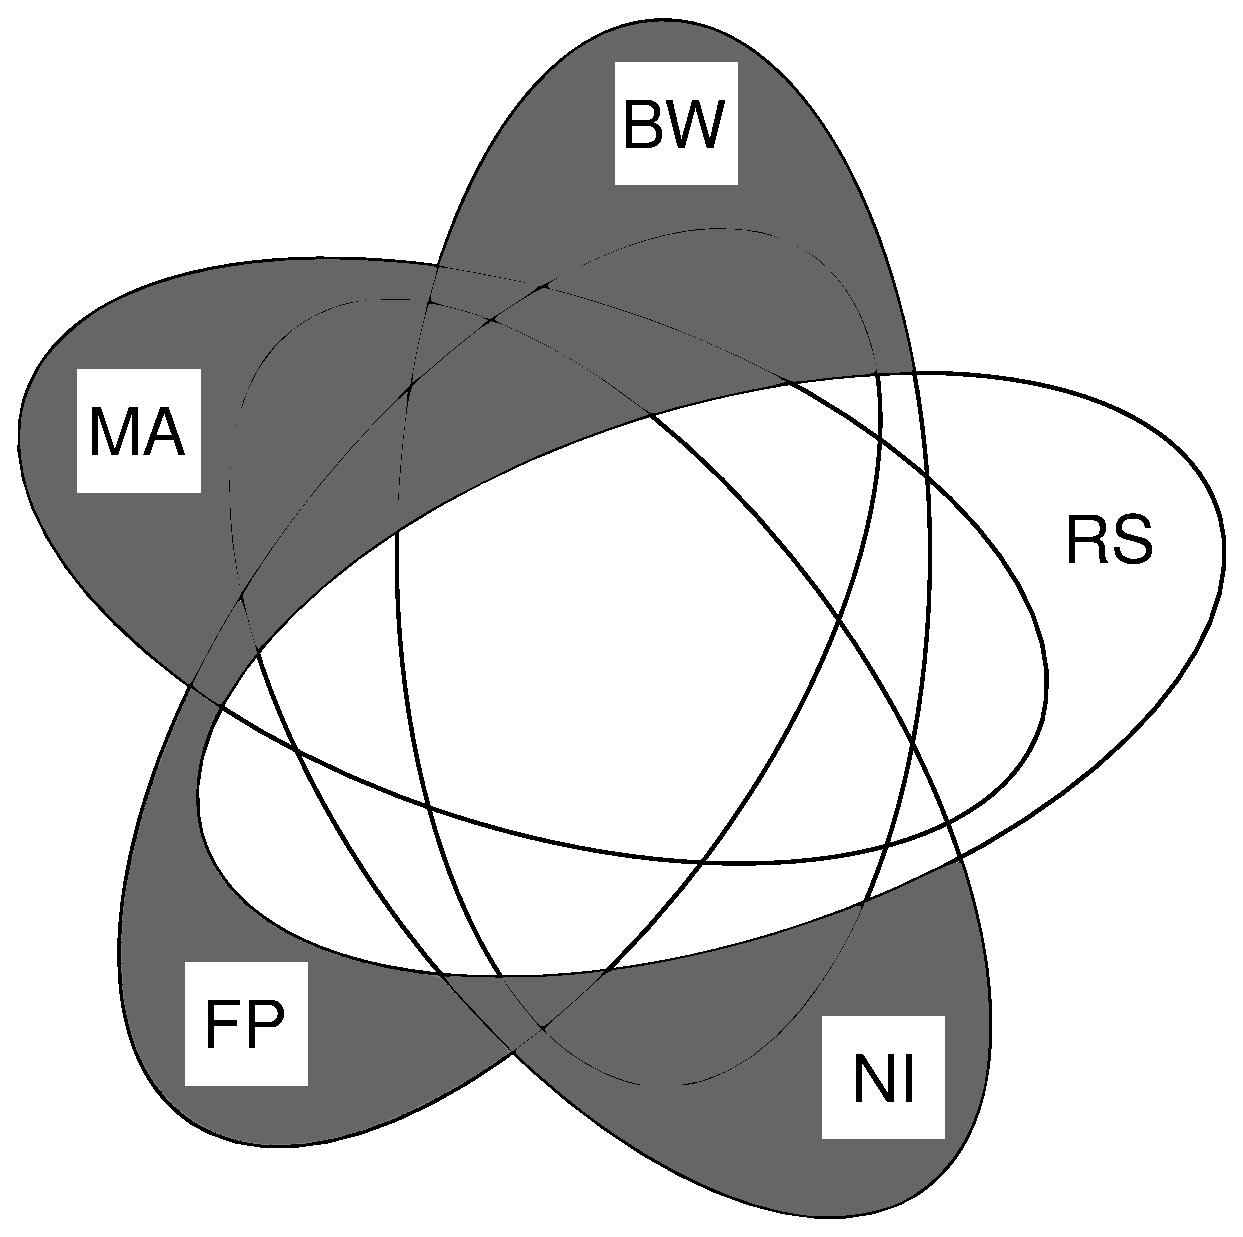
\includegraphics[width=0.49\columnwidth]{figs/static-mapping/venn_dp.pdf}
\caption{Variants solved by dynamic programming approach.}
\vspace{-1em}
\label{fig:venn_flow}
\end{figure}

Figure~\ref{fig:dynamic_motivation} \emph{(right)} shows a different node
mapping~$\NodeMapping_2$, which seeks to minimize the communication costs
between the nodes, and places all nodes in one subtree. The distance between all
nodes is two, which results in a total bandwidth allocation of~$12\cdot\CostCom$
for the interconnect. However, this reduced price comes at additional costs in
the access network:~$c_3$ and~$c_4$ have to be communicated to~$v_3$ and~$v_4$,
which requires a total bandwidth allocation of~$8 \cdot \CostTrans$.


\begin{figure}
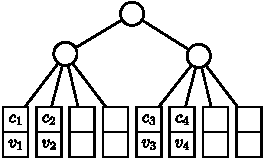
\includegraphics[width = 0.49\columnwidth]{figs/static-mapping/dynamic_bad}
\hfill
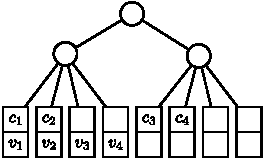
\includegraphics[width = 0.49\columnwidth]{figs/static-mapping/dynamic_good}
\caption{Two different node placements for the same substrate graph and chunk
locations. For~$\CostTrans = \CostCom$, both solutions have an identical
footprint. In other cases, one solution outperforms the other.}
\label{fig:dynamic_motivation}
\vspace{-1em}
\end{figure}



\textbf{Basic ideas.} Our proposed approach is based on dynamic programming, and
leverages the \emph{optimal substructure property} of~$\MA+\FP+\CC+\BW$:
as we will see, optimal solutions for subproblems (namely subtrees)
can efficiently be combined into optimal solutions for larger problems.
Indeed, the~$\MA+\FP+\CC+\BW$ problem
exhibits such a structure, and we show how to exploit it to
compute efficient embeddings, even in scenarios where multiple chunks
need to be assigned to flexibly placeable nodes.

For ease of presentation we will transform the
substrate network~$\Tree$
into a binary tree, using binarization:
we clone every higher-degree node,
iteratively attaching additional clones as right children
and original children as left descendants.

As usual in dynamic programs, we define, over the structure of the tree, a
recursive formula~$f$ for
the minimal cost solution \emph{given} any possible number of nodes
embedded in a given subtree. The actual set does not matter,
due to symmetry arguments.
Our approach is to evaluate this function in a bottom-up
manner.
To finally compute the actual optimal embedding,
we traverse the computed minimal-cost path backwards
(according to
the optimal values found for~$f$ during the bottom-up computation).

Concretely, the first argument to function~$f$
is a subtree~$\Tree'$, containing a given number of
chunks~$\ChunkCount(\Tree')$,
and the
second argument is the number of nodes to be embedded in the subtree.
Function~$f$ is evaluated in a bottom up manner. We initialize the
function at each leaf~$\ell$, by~$f(T_{\ell},x) =
\infty$ for all numbers of nodes~$x$ which are larger than
the server capacity~$\capacity(\ell)$;
to calculate~$f(T_{\ell}, x)$, for~$x \leq \capacity(\ell)$, we compute the
bandwidth allocation on the uplink of~$T_{\ell}$, referred to by the function
$bw(T_{\ell},x)$:
$bw(T_l,x)=  \CostTrans \cdot~$~$|x - \ChunkCount(T_{\ell})| +$~$ \CostCom \cdot
(\Vms - x) \cdot x$,
which accounts for the bandwidth allocation on the uplink of~$T_{\ell}$. The
first
term represents the required bandwidth for the communication between the~$x$
nodes on~$\ell$, and the~$\Vms - x$ nodes in the remaining parts of the substrate
network.
The second term represents
the bandwidth, which is necessary to transport the chunks from their location to
the node which should process the data (see Lemma~\ref{lemma:uplink} for more
details).

After initialization, we proceed to compute~$f$ for non-leaf
nodes in a bottom-up manner: We split the~$x$ nodes
into two positive integer
values, and we put~$r$ on the right and~$x - r$ on the left subtree.
That is, we take the optimal cost
(given recursively) of placing~$r$ nodes in
the right subtree~$\textsc{Ri}(T')$ of~$T'$ and~$x-r$ nodes in left subtree~$\textsc{Le}(T')$ of
$T'$. Given the cheapest combination, we add the bandwidth requirements
on the uplink of~$T'$ to generate the overall costs for placing~$x$ nodes in~$T'$.
Therefore,~$f(T',x) =   \min_{0\leq r \leq x}$~$ \{  f\left(\textsc{Le}(T'),
x-r\right) +$~$
f\left(\textsc{Ri}(T'), r\right) \} + bw(T',x)$.
Again, we set~$f(T',x)$ to infinity if the required bandwidth
$bw$ exceeds the capacity~$\capacity$ of the uplink of~$T'$.


\textbf{Analysis.}
The correctness and optimality of our dynamic program
is due to the decoupling of the costs induced by the tree
structure of~$\Tree$ and the  substructure
optimality property.
The substructure optimality follows from the observation that
costs can be accounted on the uplink, and the fact
 that we check each possible node distribution.
For each substrate vertex ($n_S$ many) we have
to check the cost of all possible splits,
resulting in an overall complexity of~$\mathcal{O}(n_S \cdot n_V^2)$.
The runtime to binarize~$\Tree$ is asymptotically negligible.


\subsection{Simple Problems}

\begin{figure}
\centering
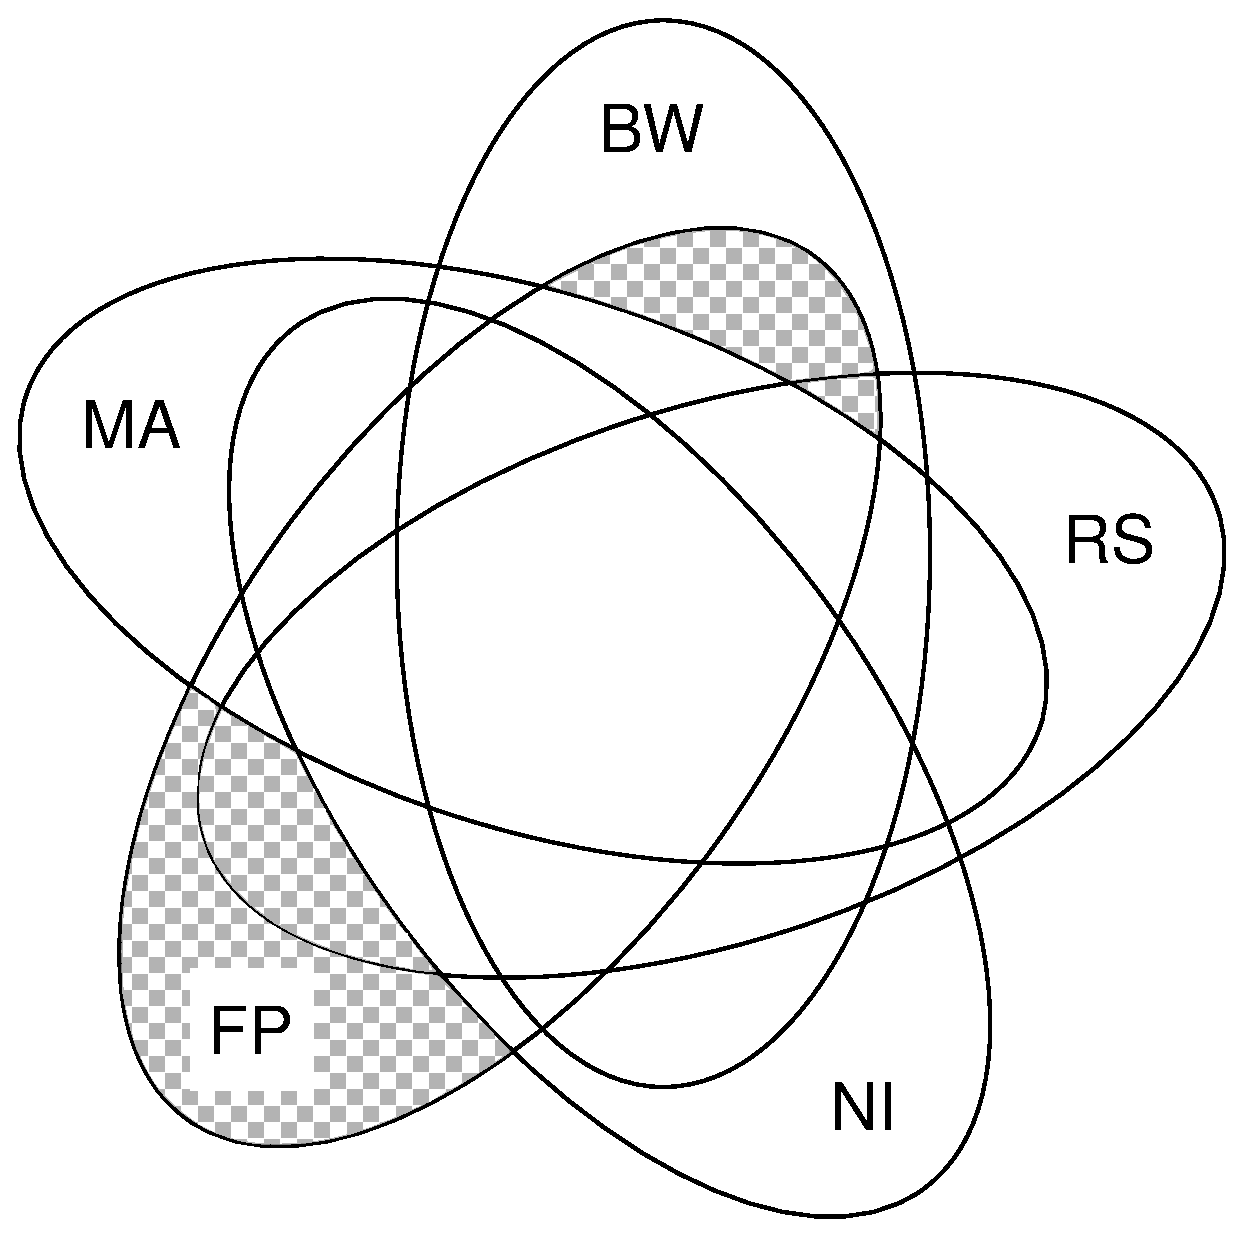
\includegraphics[width=0.49\textwidth]{figs/static-mapping/venn_trivial.pdf}
\caption{Trivially solvable problem variants.}
\label{fig:venn_trivial}
\end{figure}


For the sake of completeness, we also observe that there are
several problems which
allow for a trivial solution. Concretely, problems with~$\FP$
plus any combination of
$\RS$ and~$\BW$ (but without~$\MA$ and~$\CC$) can easily be solved by
mapping
nodes to chunk locations.
Figure~\ref{fig:venn_trivial}
shows a Venn diagram of the trivial property combinations.

%%%%%%%%%%%%%%%%%%%%%%%%%%%%%%%%%%%%%
\section{NP-Hardness Results}\label{sec:np}

We have seen that even problems with multiple dimensions of
flexibility can be solved optimally in polynomial time.
This section now points out fundamental
limitations in terms of computational tractability.
In particular, we
will show that problems become NP-hard if flexibly placeable nodes ($\FP$) have to be assigned to one of multiple replicas ($RS$), either with multiple chunks per node ($\MA$ in Section~\ref{ssec:fprsma}) or with communication among nodes ($\CC$ in Section~\ref{ssec:fprscc}).
Both results hold even in uncapacitated networks, and even in small-diameter
substrate networks (namely two- or three-level trees~\cite{fattree}).
The hardness of~$\FP+\RS+\MA$ and~$\FP+\RS+\CC$ imply
the hardness of four additional, more general models, as
summarized in Figure~\ref{fig:np_implications}:\\
\begin{figure}[htbp]
\centering
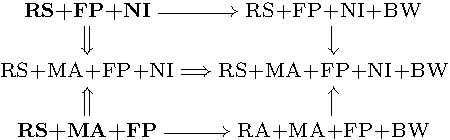
\includegraphics[width = .6\columnwidth]{figs/static-mapping/np_implications}
\caption{The NP-hardness of~$2$ variants implies the hardness of 
$4$ other variants.}
\label{fig:np_implications}
\end{figure}

\subsection{Introduction to 3D Perfect Matching}
\label{sec:3dm_intro}

Both the hardness of~$\FP+\RS+\MA$ and~$\FP+\RS+\CC$ are shown by a reduction
from the NP-complete problem of \emph{3D Perfect Matching}~\cite{3dmatch},
which we can see as a generalization of bipartite matchings to 3-uniform
hypergraphs. We will refer to this problem by~$\TDM$, and for completeness,
review it quickly:
$\TDM$ is defined as follows. We are given three finite and disjoint
sets~$X$,~$Y$, and~$Z$ of cardinality~$k$, as well as a subset of triples~$T\subseteq
X \times Y \times Z$, and $t=|T|$.  Set~$M \subseteq T$ is a 3-dimensional matching
if and only if, for any two distinct triples~$t_1=(x_1, y_1, z_1) \in M$
and~$t_2=(x_2, y_2, z_2) \in M$, it holds that~$x_1\neq x_2$,~$y_1\neq
y_2$, and~$z_1\neq z_2$. Our goal is to decide if we can construct
a~$M \subseteq T$ which is \emph{perfect}, that is, a subset which covers all
elements of~$X \cup Y \cup Z$ exactly once.


\subsection{Hardness of Multi-Assignments}\label{ssec:fprsma}

Our proof that~$\FP+\RS+\MA$ is NP-hard is based on the following main ideas.
We encode a~$\TDM$ instance as an~$\FP+\RS+\MA$ instance as follows:

 \begin{itemize}
 \item For every element in the universe~$X\cup Y\cup
 Z$, we create a chunk type. Intuitively, in~$\TDM$,
 each element must be covered, which corresponds to the requirement
 of~$\FP+\RS+\MA$
 that each chunk type is processed.

 \item We will encode each triple as gadget with three leaves in
 a substrate tree~$\Tree$. The three leaves are close to each
 other in~$\Tree$, and the placement of chunk replicas in~$\FP+\RS+\MA$
 corresponds to the elements of the
 triples in these leaves.

 \item The node placement will correspond to the choice of triples,
 independently of which
leaf the node is mapped to.
 A node will process its collocated chunk,
 as well as the chunks in other two leaves of the same gadget.

\item In order to turn the optimization problem into a decision problem, we will use
a cost threshold~$\Thr$. The cost threshold will be met by all
assignments which assign all three chunks of each triple to a
node which is collocated with one of the chunks. Assignments which connect a
chunk to a node in a different triple, will have a larger footprint, and are
considered to be infeasible.

\end{itemize}


\textbf{Construction.}
Let~$I$ be an instance of~$\TDM$ with $t$ triples and set cardinality $k$ ($k = |X| = |Y| = |Z|$).
We construct an instance~$I'$ of
$\FP+\RS+\MA$ as follows:
\begin{itemize}
\item \emph{Tree Construction:} We create a tree consisting of a root,
and for each triple, we create a gadget which we directly attach as
child of the root. The gadget is of height 2,
and has the following form:
The gadget of each triple consists of an inner node (a router) and three leaves.
\item \emph{Chunks and chunk replicas:} For each element in~$X$,~$Y$ and~$Z$,
 we create a chunk type
($3 \cdot k$ in total). Every gadget contains three chunk replicas,
corresponding to the elements of the triple. Each leave in a gadget, contains
exactly one replica.
\item \emph{Other properties:} We set the number of to-be-embedded nodes to~$k$,
$\CostTrans$ to~$1$, and the number of chunk slots in each node to the multi-assignment factor
$\MaFactor=3$.
We use a threshold~$\Thr= 4
\cdot k$.
\end{itemize}

\textbf{Example.} Figure~\ref{fig:fprsma} shows an example of our construction: An
instance~$I$ of 3-DM is given: The disjoint sets~$X$,~$Y$ and~$Z$ have a
cardinality~$k=2$. We will refer to the two elements in~$X$ as~$x_1$ and~$x_2$,
and use the same notation for the other two sets.~$T$ contains the three triples
$(x_1, y_1,
z_1)$,~$(x_2, y_1, z_2)$, and~$(x_2, y_2, z_2)$. The goal of 3-DM is to find a
subset~$M \subseteq T$, which contains each element in each of the three sets
exactly once. This instance only has one solution:~$M =
\{(x_1,y_1,z_1),(x_2,y_2,z_2))\}$.

To construct the corresponding instance~$I'$ of~$\FP+\RS+\MA$, we
create a gadget for each triple in~$T$. For each variable which occurs in a
triple, the corresponding gadget contains a chunk of the
type of the variable. The triple
$(x_2, y_1, z_2)$ of the instance is represented by the middle gadget in
Figure~\ref{fig:fprsma}. The objective of~$I'$ is to spawn~$k=2$ nodes,
with the smallest possible footprint. If the total footprint is at most $4\cdot k$, we can construct a solution to~$I$ from the solution to~$I'$.
The footprint consists of the costs which occur when a node is embedded in a
gadget, and the three chunks of that gadget which are assigned to that node: one of
the chunks is collocated with the node, the other two have to be transferred
via two hops, inflicting unitary costs on each hop.
\begin{figure}[t]
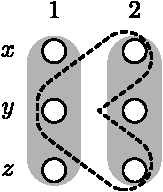
\includegraphics[width = 0.3\columnwidth]{figs/static-mapping/np_3dm_formular}
\hfill
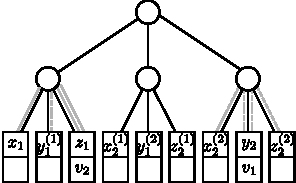
\includegraphics[width = 0.6\columnwidth]{figs/static-mapping/np_3dm_construction}
\caption{\textit{Left:} A~$\TDM$ instance with three triples:
$(x_1, y_1, z_1)$,~$(x_2, y_1, z_2)$, and~$(x_2, y_2, z_2)$. The solution is
indicated by the grey triples; the dashed triple is not used for the
solution. \textit{Right:} The corresponding problem and solution of~$\FP + \MA
+ \RS$.}
\label{fig:fprsma}
\end{figure}


\textbf{Correctness.}
Given these concepts, we can now show the computational hardness.
\begin{theorem}
$\FP+\RS+\MA$ is NP-hard.
\end{theorem}
\begin{proof}
Let~$I$ be an instance of~$\TDM$ and let~$I'$ be an instance of
$\FP+\RS+\MA$ constructed as described above. We prove that~$I'$ has a solution of cost~$\leq \Thr$ if ($\Rightarrow$) and only if
($\Leftarrow$)
$I$ has a matching of size~$k$.

($\Rightarrow$) Let us take a feasible solution to~$\TDM$. We place a node in every
gadget that corresponds to the chosen triples. In each of the corresponding
gadgets, we match every chunk to the node in this gadget. This
solution has
cost exactly~$\Thr$. As every element of the universe is covered, every
chunk type is processed.

($\Leftarrow$) Let us take a solution to~$\FP+\RS+\MA$ of cost at most$\Thr$. We
choose triples that correspond to gadgets where there are nodes. Since
all chunks are processed, every element of~$X$,~$Y$ and~$Z$ is matched. Each
node must process chunks that
correspond to the triple, otherwise the
cost must be larger than~$\Thr$ (high costs for chunk
transportation).
\end{proof}


\subsection{Hardness of Inter-connects}\label{ssec:fprscc}


Next, we prove that the joint optimization of node placement and replica selection
is NP-hard if an inter-connect has to be established between nodes.
In our terminology, this is the~$\FP+\RS+\CC$ problem.

The proof is similar in spirit to the proof of~$\FP+\RS+\MA$, however,
we modify the construction to account for the absence of~$\MA$:
we choose
a high value for~$\CostTrans$, such that nodes will be directly collocated with
their assigned chunks. We leverage the fact that any solution which does not
assign 0 or 3 chunks to each gadget, will have higher communication costs.

\textbf{Construction.}
Let~$I$ be an instance of~$\TDM$ with $t$ triples and set cardinality $k$ ($k = |X| = |Y| = |Z|$). We will create an instance~$I'$
for~$\FP+\RS+\CC$ as follows:
\begin{itemize}
\item We will construct the same tree as in previous reduction with
chunk replicas placed in the same way.
\item The communication cost in the inter-connect is set to~$\CostCom = 1$.
\item The number of nodes (virtual machines) is~$\Vms = 3 \cdot k$, where~$k$ is the set cardinality.
\item Only solutions which place a node in each leaf of~$k$ gadgets, can
be converted into solutions for the 3-DM problem. We use the cost threshold
$\Thr =  6 \cdot k + 18 \cdot
(k - 1) \cdot k$, to verify whether a solution achieves this, transforming
$\FP+\RS+\CC$ into a decision problem. A detailed explanation of this value can
be found in the proof of Theorem~\ref{theorem:fp_rs_cc}.
\item We set the access cost~$\CostTrans$ to a chunk replica to a high value~$W$. This will force
nodes to be collocated with the replica. One example of sufficient
(and polynomial but not necessarily minimal)~$W$
is the value of the threshold~$\Thr+1$. Any solution not
assigning chunks to collocated nodes, have cost~$> \Thr$:
communicating a chunk inflicts costs~$W=\Thr+1$ over every link.
\end{itemize}

We focus on instances with unit server capacities.

\textbf{Proof of correctness of the reduction.}
Intuitively, in order to minimize embedding costs,
nodes should be placed on near-by replicas. We use the following
helper lemma.
\begin{lemma}\label{lemma:helper}
In every valid solution of~$I'$ of cost~$\leq \Thr$, each gadget
falls in one of two categories:
$k$ gadgets have exactly
$3$ nodes, and~$t-k$ gadgets remain empty.
\end{lemma}
\begin{proof}
Since~$W$ is large enough, the~$3\cdot k$ nodes have to be placed
directly on different chunks, resulting in 0 costs for the access network.
Consider any pair of nodes
communicating over the
inter-connect; due to our construction, the communication cost
for each such pair is either
2 hops (if they belong to the same gadget) or 4 hops (if they belong
to different gadgets).
The lemma then follows from the observation that~$\Thr$
is chosen such that it is never possible to distribute nodes
among more than~$k$ gadgets.
\end{proof}

\begin{theorem}
\label{theorem:fp_rs_cc}
$\FP+\RS+\CC$ is NP-hard.
\end{theorem}
\begin{proof}
Let~$I$ be an instance of~$\TDM$ and let~$I'$ be an instance of
$\FP+\RS+\CC$ constructed as described above.
We prove that~$I'$ has solution of cost~$\leq \Thr$ if ($\Rightarrow$) and only if
($\Leftarrow$)
$I$ has a solution.

($\Rightarrow$) In order to compute a solution
for~$I'$ given a solution for~$I$, we proceed as follows.
Given an exact covering set of triples~$S = \{t_1, t_2,
\ldots, t_k\}$, we place three nodes in each gadget that
corresponds to every triple of~$S$. Chunks are matched to the nodes which are located
on the same server.

The solution has the following cost:
(1) the communication cost inside a gadget is~$2 \cdot {3 \choose 2}$,
  as every pair contributes two hops;
  (2) the communication cost from each gadget to all other gadgets is~$4
  \cdot 3 \cdot 3 \cdot (k - 1) / 2$, where the factor~$4$ is
  for the
  communication over~$4$ hops, the factor~$3$
  corresponds to the number of nodes per gadget, and
 ~$3 \cdot (k-1)$ is the number of nodes in remote gadgets;
  as we count each pair twice, we need to divide by two in the end.
Summing up over all~$k$ gadgets, we get exactly~$\Thr$.

($\Leftarrow$) Given a solution for~$I'$,
we can exploit Lemma~\ref{lemma:helper} to construct a solution for~$I$.
We know that in any solution of cost at most~$\Thr$,
$k$ gadgets contain exactly 3 nodes. These gadgets correspond to a valid
3D Perfect Matching: exactly one replica of every chunk type is processed and
hence every element is covered exactly once.
\end{proof}


\section{A Detailed Study of Replica Selection Hardness}\label{ap:tworep}
We have seen that replica selection flexibilities can render embeddings computationally hard.
We will now provide a more detailed look at this hardness result
and explore the minimal requirements for rendering replica selection hard.
In particular, we will show that already two replicas for each chunk type are sufficient to
introduce intractability.

Namely, we provide the NP-hardness results for two restricted variants of Virtual Cluster Embedding (Sections~\ref{ap:tworep-ma} and \ref{ap:tworep-ni}).
We augment the $\RS$ variant of $\VCEMB$ problem in the following way: by $\RS(k)$ we denote the problem where each chunk has the redundancy factor at most $k$.
In Section~\ref{ap:tworep-ma} we provide the hardness result for $\RS(2)+\MA+\FP$, and in Section~\ref{ap:tworep-ni} we provide the hardness result for $\RS(2)+\FP+\CC+\BW$.

Both problems are reduced from the problem $\TDPM$ (see Section~\ref{sec:3dm_intro} with no further restrictions.
The constructions are based upon the reduction of $\TDPM$ to $\FP+\RS+\MA$ (see Section~\ref{ssec:fprsma}) and the reduction of $\TDPM$ to $\FP+\RS+\CC$ (see Section~\ref{ssec:fprscc}).
However, in contrast to Section~\ref{ssec:fprscc}, in two replica variant without multiple assignment, we added the bandwidth constraints.
It is currently unknown to the authors of this very paper, whether the hardness result holds without bandwidth constraints (namely, whether the problem $\RS(2)+\FP+\CC$ is NP-hard).
The necessity for bandwidth constraints arises as to deal with restricted factor of replication, we need to introduce gadgets in the tree that makes the tree asymmetric.
Introducing bandwidth constraints allows to control the number of nodes spawning in certain parts of the tree.

\subsection{Two Replicas without Bandwidth Constraints}\label{ap:tworep-ma}

We now show that the 2-replica selection problem is even NP-hard
without capacity constraints.  In particular, we consider the problem
variant~$\RS(2)+\MA(4)+\FP$ with at most two replicas of each chunk type and assignment factor
four. There are no capacity constraints on links.

Our construction consists of two major modifications to hardness result without replication factor restrictions (for that result, refer to Section~\ref{ssec:fprsma}).

\textbf{Unique chunks on the comb.} First, we provide the tools for restricting the placement of nodes in certain parts of the tree.
In Section~\ref{ssec:fprsma}, due to symmetric structure of the tree, the carefully crafted threshold value allowed us to prove that e.g. no Triple Gadget ever had two or more nodes placed in it.
We still use the threshold value as the placement mechanism, but in this section, due to the asymmetrical tree construction, we combine it with the concept of unique chunks on the comb (by \emph{comb} we denote the balanced tree, where all non-root vertices have at most one child).

For an introduction to the concept of unique chunks, let us consider the following example.
Suppose that within one $\VCEMB$ construction, we would like to encode not one $\TDPM$ instance, but two $\TDPM$ instances: $M_1$ and $M_2$, with disjoint universe and different number of triples to be chosen: $n_1$ and $n_2$.
We perform the following modifications to the encoding provided in Section~\ref{ssec:fprsma}.
The multi-assignment factor grows by $1$, that is the instance we construct is the $\RS+\MA(4)+\FP$ instance.
We construct two subtrees $T_1$ and $T_2$, that correspond to $M_1$, resp. $M_2$; we construct two two-edge-level combs $C_1$ and $C_2$, with number of leaves $n_1$, resp. $n_2$.
We attach $M_1$ and $C_1$ (resp. $M_2$ and $C_2$) to the common root and we name the resulting subtree $P_1$, resp. $P_2$.
Next, we attach $P_1$ and $P_2$ to the common root.
In the end, the height of the tree grew by $2$.
Finally, we populate both combs with unique chunks, and we set the number of to-be-placed nodes to $\Vms = n_1+n_2$.
We modify the threshold to be the sum of the thresholds for constructions for $M_1$ and $M_2$ plus $4\cdot (n_1 + n_2)$.
The last substrate of the threshold value corresponds to transportation of the fourth chunk processed by each machine for the distance of four.

To see why the example indeed can solve two instances of $\TDPM$, we need the following observations.
First, we claim that no node is ever placed in a comb.
To prove this fact, we use the property of the comb that the leaves are highly separated, and the fact that each machine has to process $4$ chunks.
Next, we claim that the number of nodes spawned in $P_1$ (resp. $P_2$) is $n_1$ (resp. $n_2$).
To see this, consider any imbalance of the number of spawned nodes; notice that some chunks in the underpopulated comb are processed outside of their $P_i$ subtree, resulting in the solution that exceeds the threshold.

\textbf{Families of chunk types.} The second tool that we introduce allows us to express the redundancy of chunks without actually replicating chunks more than two-fold.
For simplicity of introduction, we consider the scenario with no multi-assignment.
For each chunk type $c$ with redundancy, we count the number of occurrences of replicas of such a chunk in the tree, and name it $r_c$.
We replace the chunk type $c$ with $r$ chunk types, which we call the family $F_c$ of that chunk type.
For each occurrence of replica of $c$, we replace it with a replica of any chunk type from the family (without repetitions).
To this point, the redundancy factor was reduced from $r_c$ to $1$.
Now, we construct the gadget $G_c$ for chunk type $c$, which consists of $r_c$ leaves, each hosting the second replica of each chunk type from family $F_c$.
We use the technique of unique chunks on the comb to constraint the number of nodes in $G_c$ to be exactly $r_c - 1$.
We provide necessary additional $r_c-1$ nodes to be placed.
Hence, exactly $1$ node is placed on a chunk type of family $F_c$ outside the gadget $G_c$, and exactly $r_c-1$ nodes cover the remaining $r_c-1$ chunk types inside gadget $G_c$.
All chunk types are processed, the replication factor is reduced to $2$, and the size of construction grows polynomially.

\textbf{Introduction to the reduction.} As we already stated, we modify the construction from Section~\ref{ssec:fprsma}.
As a way to deal with replication, we use the families of chunk types using the unique chunks on the comb.
We extend the construction of a gadget for chunk type with redundancy, by incorporating the fact that the multi-assignment factor is $4$.
For the construction to remain correct given such a multi-assignment factor, we introduce further chunks types with one chunk replica to place in the chunk gadget and use the excessive $3$ data processing capacities.

\textbf{Construction.}
For arbitrary instance~$I_{\TDPM}$ of~$\TDM$ we construct a~$\RS(2)+\MA(4)+\FP$ instance~$I_{\VCEMB}$ the way described in the remainder of this section.
Let $k = |X|=|Y|=|Z|$.

By $T$ we denote the set of all triples of $I_{\TDPM}$, and let $t = |T|$.
For each $e\in X\cup Y\cup Z$, by $T_e$ we denote the set of all triples that contain element $e$.
Let $\deg(e) = |T_e|$, and note that $\sum_e \deg(e) = 3\cdot t$.

We proceed with the construction as follows.

\paragraph{Chunk types and replicas}

We construct three sets of chunk types.
The first set corresponds to elements of the universe (that is, $X\cup Y\cup Z$).
The construction of such chunk types is similar to construction of chunk types in Section~\ref{ssec:fprsma}, but to take into consideration the restricted replication factor, we construct the familiy of chunk types (as described in the introduction to this section).
Namely, for each element of universe $e$, we construct as many chunk types as there are occurences of $e$ in triples of $I_{\TDPM}$.
Each such chunk type has exactly two replicas.

The other two sets of chunk types has one replica, therefore those are called called \emph{unique} chunks.
We construct two types of unique chunks, distinguished by a different role in the construction.
For unique chunks we simply co-notate the chunk type with chunk replica.

Formally, the construction of chunk types and replicas unfolds as follows:
\begin{enumerate}
  \item For each triple $\tau \in T$, we construct $3$ chunk types, with two replicas each.
  We construct different chunk types for each triple $\tau$, which contain element $e$ (in total $\deg(e)$ chunk types).
  We refer to those replicas by $ch_1(e, \tau)$ and $ch_2(e, \tau)$.
  In total we construct $2\cdot \sum_e\deg(e) = 6\cdot t$ chunk replicas.
  \item We construct~$k$ additional chunk types named
  ~$u_1, \ldots, u_k$ with one replica each.
  \item For each element~$e\in X\cup Y\cup Z$,
  we construct additional~$3\cdot(\deg(e) - 1)$ chunks, with one replica each.
  We call this set~$\UniqueE$.
\end{enumerate}

\paragraph{Tree.}

\begin{figure}[t]
  \centering
  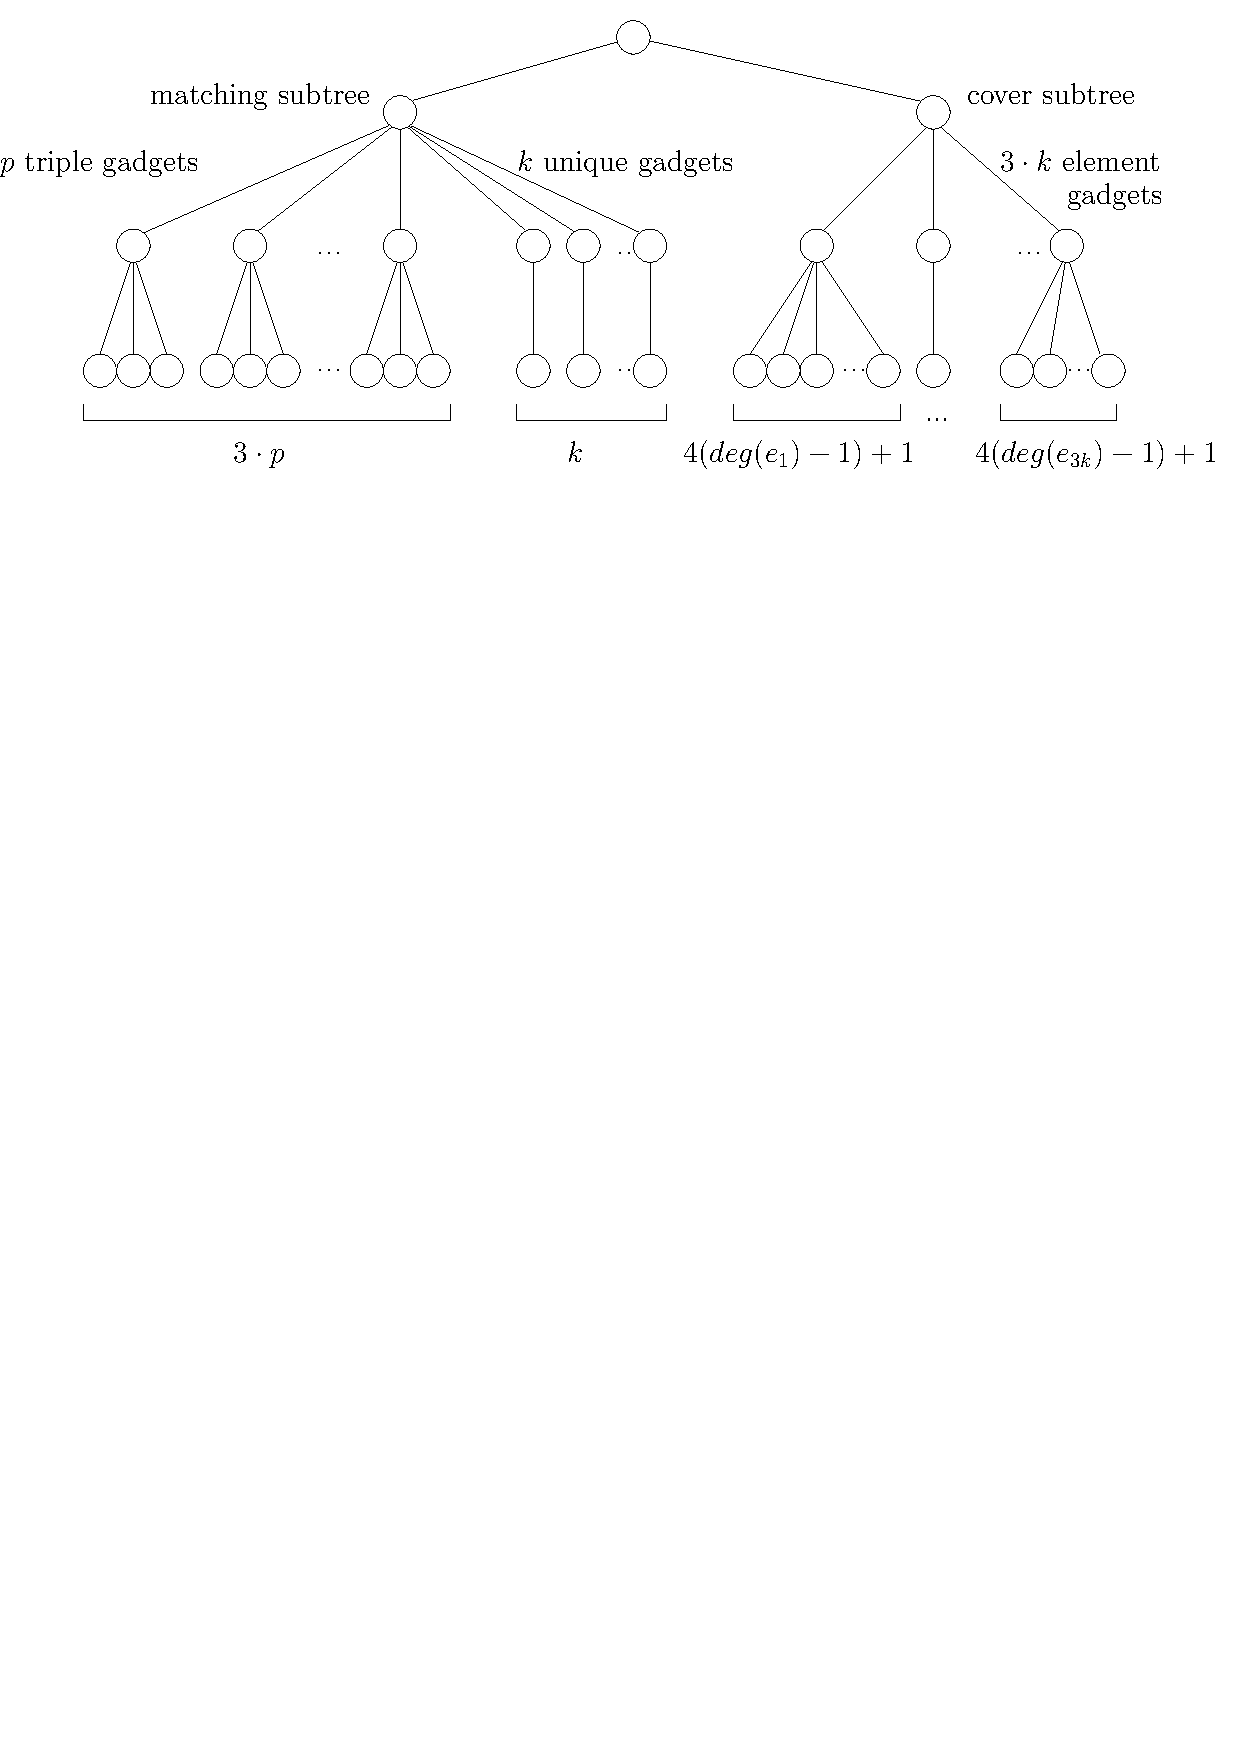
\includegraphics[width=0.99\columnwidth]{figs/static-mapping/overview}
  \vspace{-1em}
  \caption{Overview of the substrate network}
  \vspace{-1em}
  \label{fig:red-ma2}
\end{figure}


We construct the tree that has the following structure (see Figure~\ref{fig:red-ma2}):

\begin{enumerate}
  \item The physical network consists of two subtrees connected to the
  root: the {\MatchSubtree} and the {\CoverSubtree}. The
  {\MatchSubtree} consists of $t$ {\TripleGadgets}, one per each triple $\tau\in T$ and $k$
  {\UnqGadgets}. The {\CoverSubtree} consist of~$3\cdot k$ {\ElGadgets}, one for each element $e\in X\cup Y\cup Z$.
  \item {\TripleGadget} consists of four vertices: three leaves and the root of the gadget.
  \item {\UnqGadget} consists of two vertices: the leaf and the root of the gadget.
  We construct the root node of the gadget not only to keep the tree balanced, but also to keep leaves of
  {\UnqGadgets} far from leaves of other \UnqGadgets. Note that \UnqGadgets{} form a comb.
  \item {\ElGadget} for element $e$ has a structure that depends on the number of triples that cover $e$. The {\ElGadget} consists of the
  root and~$4\cdot(\deg(e)-1)+1$ leaves.
\end{enumerate}

\paragraph{Chunk Placement.}
The chunks are placed as follows:
\begin{enumerate}
  \item \emph{Chunks in the Matching Subtree:} In {\TripleGadget} of triple $\tau$ we put
  three replicas:
 ~$ch_1(e_X(\tau), \tau), ch_1(e_Y(\tau), \tau), ch_1(e_Z(\tau), \tau)$, one per each leaf.
  \item \emph{Chunks in the Unique Gadgets:} We place replicas
 ~$u_1,\ldots, u_k$ at the leaves of \UnqGadgets.
 \item \emph{Chunks in Element Gadgets:} Consider the \ElGadget{} for the element $e \in X\cup Y\cup Z$.
 We place two types of replicas in the leaves of the gadget.
 We put replicas $ch_2(\tau, e)$ for each $\tau \in T_e$.
 Additionally, we place all the replicas from set $\UniqueE$.
 In total, we place $4\cdot (\deg(e) - 1) + 1$ replicas, one per each leaf of the gadget.
\end{enumerate}

\paragraph{Other properties of the instance.}
\begin{enumerate}
  \item \emph{Multiple assignment:} We set the multi-assignment factor to $m=4$.
  \item \emph{Number of nodes:} We set the number of nodes to spawn to
 ~$\numNodes = k + \sum_{e}(\deg(e)-1) = 3\cdot t - 2\cdot k$ nodes.
 \item \emph{Threshold:} We set the following threshold:
 ~$\Thr = 18\cdot t - 10\cdot k$.
 This value corresponds to the cost of solution, where $k$ nodes are matched to $4$ chunks that are in distance: $0, 2, 2$ and $4$ to the node, and remaining $\Vms-k$ nodes are matched to $4$ chunks that are in distance: $0, 2, 2$ and $2$ to the node.
\end{enumerate}

\textbf{The reduction.}

Given any $\TDPM$ instance $I_{\TDPM}$, we produce corresponding instance of $\VCEMB$ variant, namely the $\RS(2)+\MA+\FP$ instance, in the way described above.
We refer to such $\RS(2)+\MA+\FP$ instance as the $I_{\VCEMB}$.

The reduction (Theorem~\ref{th:ma-reduction}) unfolds in two stages.
First, given a solution $S_{\TDPM}$ to $I_{\TDPM}$, we construct a solution $S_{\VCEMB}$ to $I_{\VCEMB}$.
This part is the easier of the two, and mainly consists of placing nodes in Triple Gadgets for triples chosen in $S_{\TDPM}$.

In the second stage, given $S_{\VCEMB}$, we construct the $S_{\TDPM}$.
In this stage, the main difficulty lies in showing that $S_{\VCEMB}$ has certain structure.

We call the {\TripleGadget} \textit{active}, if it contains a node at any leaf, and we call the node \textit{active} if it is placed in {\TripleGadget}.
Our goal is to show that in every feasible solution, exactly $k$ \TripleGadgets{} are active (Lemma~\ref{lem:n-active-ma}), and hence we can construct $S_{\TDPM}$ from the triples that correspond to active \TripleGadgets{} in $S_{\VCEMB}$.

In $I_{\VCEMB}$, chunks can be matched to nodes at distance $0, 2, 4$ or $6$.
  We call the matches at distance $0$ the \emph{free matches}, the matches at distance $2$ the \emph{neighbouring matches}.
  In addition we call the matches at distance $0$ or $2$ the \emph{short matches}, and the matches at distance $4$ or $6$ the \emph{long matches}.
  We call the distance between the pair of leaves the \emph{short distance}, if the distance between them is at most $2$, otherwise we call said distance the \emph{long distance}.

Proving the existance of more than $k$ long matches is sufficient to show that the instance is infeasible, as its cost exceeds the threshold.
To see this, note that the threshold value $\Thr$ corresponds to the cost of solution, where $k$ nodes has $1$ free match, $2$ neighbouring matches and $1$ long match at distance of $4$ hops, and remaining $\Vms-k$ nodes has $1$ free match and $3$ neighbouring matches assigned.
Note that the limit of $\Vms$ free matches is exhausted, hence excessive long matches cannot be compensated in any way.
Hence, at most $k$ long matches are present in any feasible solution.


\begin{lemma}
  In $S_{\VCEMB}$ there are have exactly $k$ nodes spawned in the \MatchSubtree.
  \label{lem:n-matchsubtree-ma}
\end{lemma}

\begin{proof}
 We claim that each node spawned in the \MatchSubtree{} results in at least one long match.
This fact is a consequence of the structure of the tree and the fact that multi-assignment factor is set to $4$.
For each node spawned in the \MatchSubtree{}, by the construction of the tree, the node has at most $3$ leaves in short distance, hence at least one of the matches is long.
Hence, we conclude that spawning more than $k$ nodes in the \MatchSubtree{} results in more than $k$ long matches, which results in infeasibility of the solution.
In addition, each node spawned in \UnqGadget{} results in at least $3$ long matches, as the only leaf in short distance is the leaf collocated with the node.

As at most $k$ nodes are spawned in \MatchSubtree{}, at least $\Vms-k$ nodes are spawned in the \CoverSubtree.
Assume then that $\Vms-k+i$ nodes spawned in the \CoverSubtree{} for non-negative $i$.
Now, we argue that such node configuration results in $3\cdot i$ long matches.
Consider the \ElGadget{} $g_e$ for element $e$.
The gadget $g_e$ has exactly $4\cdot(\deg(e)-1)+1$ leaves, each hosting exactly one chunk replica.
As $4\cdot(\deg(e)-1)+1 \mod 4 = 1$, spawnining $\deg(e)-1+j$ nodes in $g_e$ for non-negative $j$ results in at least $3\cdot j$ long matches by the fact that there are insufficient chunk replicas in the short distance.
Using the fact that $\sum_e(\deg(e)-1) = 3\cdot t - 3\cdot k = \Vms - k$, by pidgeon-hole principle we conclude that indeed spawning $\Vms-k+i$ nodes in the \CoverSubtree{} results in at least $3\cdot i$ long matches.

Consider the configuration with $\Vms-k+i$ nodes spawned in the \CoverSubtree{}, and $k-i$ nodes spawned in the \MatchSubtree{}.
Such configuration results in at least $2\cdot i + k$ long matches, where $3\cdot i$ long matches come from the excessive nodes spawned in the \CoverSubtree{}, and $k-i$ long matches come from $k-i$ nodes in the \MatchSubtree{}.
Hence we deduce that $i = 0$, as otherwise the number of long matches would exceed $k$.

\end{proof}

\begin{lemma}
  In $S_{\VCEMB}$ no node spawned in \UnqGadget{}.
  \label{lem:no-unq-ma}
\end{lemma}
\begin{proof}
  By Lemma~\ref{lem:n-matchsubtree-ma}, exactly $k$ nodes spawned in the \MatchSubtree{}.
Suppose that out of $k$ nodes in the \MatchSubtree{}, a non-negative number of nodes $j$ spawned in the \UnqGadgets{}.
From the fact that each leaf of \UnqGadget{} has long distance to every other leaf, every node spawned in \UnqGadget{} result in at least $3$ long matches.
Hence, the total number of long matches is at least $k-j + 3\cdot j$.
Finally, for the solution to be feasible we allow at most $k$ long matches, therefore no node spawns in the \UnqGadget{}.
\end{proof}

\begin{lemma}
  In $S_{\VCEMB}$ there are have exactly $k$ active \TripleGadgets{}.
  \label{lem:n-active-ma}
\end{lemma}
\begin{proof}
  By Lemmas~\ref{lem:no-unq-ma} and \ref{lem:n-matchsubtree-ma} we conclude that $k$ nodes spawned in the \TripleGadgets.
As there are exactly $3$ replicas in each \TripleGadget{}, spawning more than one node in a single \TripleGadget{} results in at least additional $3$ long matches.
Hence, exactly $k$ \TripleGadgets{} are active.
\end{proof}

\begin{lemma}
  In $S_{\VCEMB}$ every chunk replica besides $u_1, \ldots, u_k$ is matched by a short match.
  \label{lem:short-ma}
\end{lemma}
\begin{proof}
  By Lemma~\ref{lem:n-active-ma}, exactly $k$ nodes are spawned in \TripleGadgets{}, and by Lemma~\ref{lem:no-unq-ma} we deduce that chunks $u_1, \ldots, u_k$ are matched by long matches.
  As at most $k$ long matches are allowed for the solution to be feasible, remaining matches are short.
\end{proof}

\begin{theorem}
  ~$\RS(2)+\MA+\FP$ is NP-hard.
  \label{th:ma-reduction}
\end{theorem}

\begin{proof}
  
  Let's take any instance $I_{\TDPM}$ of~$\TDPM$.
  We show that~$I_{\VCEMB}$ has a solution of cost~$\leq \Thr$ if and only if~$I_{\TDPM} \in \TDPM$ (there exists a perfect 3D matching in $I_{\TDPM}$).

  ($\Leftarrow$) Let's take any feasible solution~$S_{\TDPM}$ to $I_{\TDPM}$.
  We construct a solution~$S_{\VCEMB}$ in the following way:
  \begin{enumerate}
    \item We place~$k$ nodes in~$k$ {\TripleGadgets} (one per gadget) that correspond to triples in~$S_{\TDPM}$.
    The choice of exact leaf of the gadget to place a node is arbitrary.
    We match each such node to $3$ chunk replicas in the gadget it is placed, and we match $1$ arbitrary, unmatched chunk replica in {\UnqSubtree}.
    \item In each {\ElGadget} that corresponds to element~$e$, we place
   ~$\deg(e) - 1$ nodes and match them to arbitrary chunks in this
    gadget, which are not yet matched in any {\TripleGadget}.
  \end{enumerate}

  We can observe that every chunk type was processed, exactly $k + \sum_e(\deg(e) - 1)$ nodes are spawned, and each of the nodes process exactly $4$ chunk replicas.
  To see that indeed the produced solution do not exceed the threshold $\Thr$, we sum up the total transportation cost.
  The $k$ nodes placed in \TripleGadgets{} have $1$ free match and $2$ neighbouring matches to chunk replicas within the \TripleGadget{}, and $1$ long match of cost $4$ (to some \UnqGadget{}).
  The remaining $\Vms-k$ nodes placed in the \CoverSubtree{} have $1$ free match and $3$ neighbouring matches.
  In total, the cost incurred is $8\cdot k + 6\cdot (\Vms - k) = \Thr$.
  Hence, the solution is indeed feasible.

  ($\Rightarrow$) Let's take any feasible solution~$S_{\VCEMB}$ to~$I_{\VCEMB}$ in the way described in the construction section.
  By Lemma~\ref{lem:n-active-ma}, exactly $k$ \TripleGadgets{} are active.
  We construct the solution $S_{\TDPM}$ from the set of triples that correspond to active \TripleGadgets{}.

  It remains to show that $S_{\TDPM}$ indeed matches every element of $X\cup Y\cup Z$.
  By Lemma~\ref{lem:short-ma}, each match of $ch(e, \tau)$ for each $e\in X\cup Y\cup Z$ and each $\tau \in T$ is matched by a short match.
  Hence, each active node processes the 3 chunks that are placed in its \TripleGadget.
  In each {\ElGadget} for element~$e$, one chunk $ch(e, \tau)$ for some $\tau \in T$ is not matched.
  Let's call this chunk instance~$\Unmatched(e)$, and let's call~$\Unmatched = \cup_e \Unmatched(e)$.
  Note that~$|\Unmatched| = 3\cdot k$.
  The set~$\Unmatched$ is covered by \ActiveNodes{}, and hence the set of triples in $S_{\TDPM}$ form a 3D Perfect Matching of $X\cup Y\cup Z$.
\end{proof}


\subsection{Two replicas without Multiple Assignment}\label{ap:tworep-ni}

We now show that~$\RS(2)+\FP+\CC+\BW$ is even NP-hard without multiple
assignment.
The proof is similar in spirit to proof of hardness of $\RS(2)+\FP+\MA$.

The reduction (Theorem~\ref{th:ma-reduction}) unfolds in two stages.
First, given a solution $S_{\TDPM}$ to $I_{\TDPM}$, we construct a solution $S_{\VCEMB}$ to $I_{\VCEMB}$.
This part is the easier of the two, and mainly consists of placing nodes in Triple Gadgets for triples chosen in $S_{\TDPM}$.

In the second stage, given $S_{\VCEMB}$, we construct the $S_{\TDPM}$.
Again, we use the technique that we call ``families of chunk types'', which was introduced in previous section.
The main technical difficulty lies in controlling the number of nodes that are spawned in certain parts of (asymmetric) tree.
To guantee the desired number of spawned nodes, we use the bandwidth constraints.
Namely, if the number of nodes to be spawned in a subtree is $k$, we set the bandwidth constraints on the uplink of the subtree to $k\cdot (m - k)$, where $m$ is the total number of machines to spawn in the instance.
As we further see in Lemma~\ref{lem:bandwidth1}, such bandwidth constraint in form of a quadratic expression provides both lower- and upper-bound on the number of machines spawned in such subtree.
To see this, consider a simple example: regardless of the bandwidth constraint on the uplink of the subtree, capacities are not exceeded in at least two scenarios: with all $m$ nodes spawned in the subtree, and with $0$ nodes spawned in the subtree.
More precisely, bandwidth constraints in such form excludes configurations with number of nodes between $k$ and $m-k$.

However, we are interested only in lower-bounding the number of nodes to spawn in a subtree, and in fact the upper-bound on the number of nodes is only a liability.
We make sure that the upper-bound on the number of nodes is always satisfied by artificially increasing the number of total nodes to be spawned.
In this way the upper-bound on number of nodes always exceeds the number of leaves of any subtree in which we would like to have $k$ nodes spawned, see Lemmas~\ref{lem:bandwidth2} and \ref{lem:bandwidth3}.
Additional nodes do not interfere with the rest of the construction, as we provide unique chunks for them to process.



\noindent \textbf{Construction.}

For arbitrary instance~$I_{\TDPM}$ of~$\TDM$ we construct a~$\RS(2)+\FP+\CC+\BW$ instance~$I_{\VCEMB}$ the way described in the remainder of this section.
Let $k = |X|=|Y|=|Z|$.
By $T$ we denote the set of all triples of $I_{\TDPM}$, and let $t = |T|$.
For each $e\in X\cup Y\cup Z$, by $T_e$ we denote the set of all triples that contain element $e$.
Let $\deg(e) = |T_e|$, and note that $\sum_e \deg(e) = 3\cdot t$.

We proceed with the construction as follows.

\emph{Chunk Types.}
We construct two sets of chunk types.
The first set corresponds to elements of the universe (that is, $X\cup Y\cup Z$).
The construction of such chunk types is similar to construction of chunk types in Section~\ref{ssec:fprscc}, but to take into consideration the restricted replication factor, we construct the familiy of chunk types (as described in the introduction to this section).
Namely, for each element of universe $e$, we construct as many chunk types as there are occurences of $e$ in triples of $I_{\TDPM}$.
Each such chunk type has exactly two replicas.

The other set of chunk types has one replica, therefore those are called called \emph{unique} chunks.
For unique chunks we simply co-notate the chunk type with chunk replica.

Formally, the construction of chunk types and replicas unfolds as follows:
\begin{enumerate}
  \item For each triple $\tau \in T$, we construct $3$ chunk types, with two replicas each.
  We construct different chunk types for each triple $\tau$, which contain element $e$ (in total $\deg(e)$ chunk types).
  We refer to those replicas by $ch_1(e, \tau)$ and $ch_2(e, \tau)$.
  In total we construct $2\cdot \sum_e\deg(e) = 6\cdot t$ chunk replicas.
  \item Additionally, we construct
$\max\{3\cdot t + 3\cdot k + 1, \sum_e(2\cdot \deg(e)-1)\}$
chunk types called \emph{unique chunks}. We
refer to the set of unique chunks by~$U$.
\end{enumerate}

\emph{The substrate network.}
We construct the tree that has the following structure (see Figure~\ref{fig:red-cc}):

\begin{figure}[t]
  \centering
  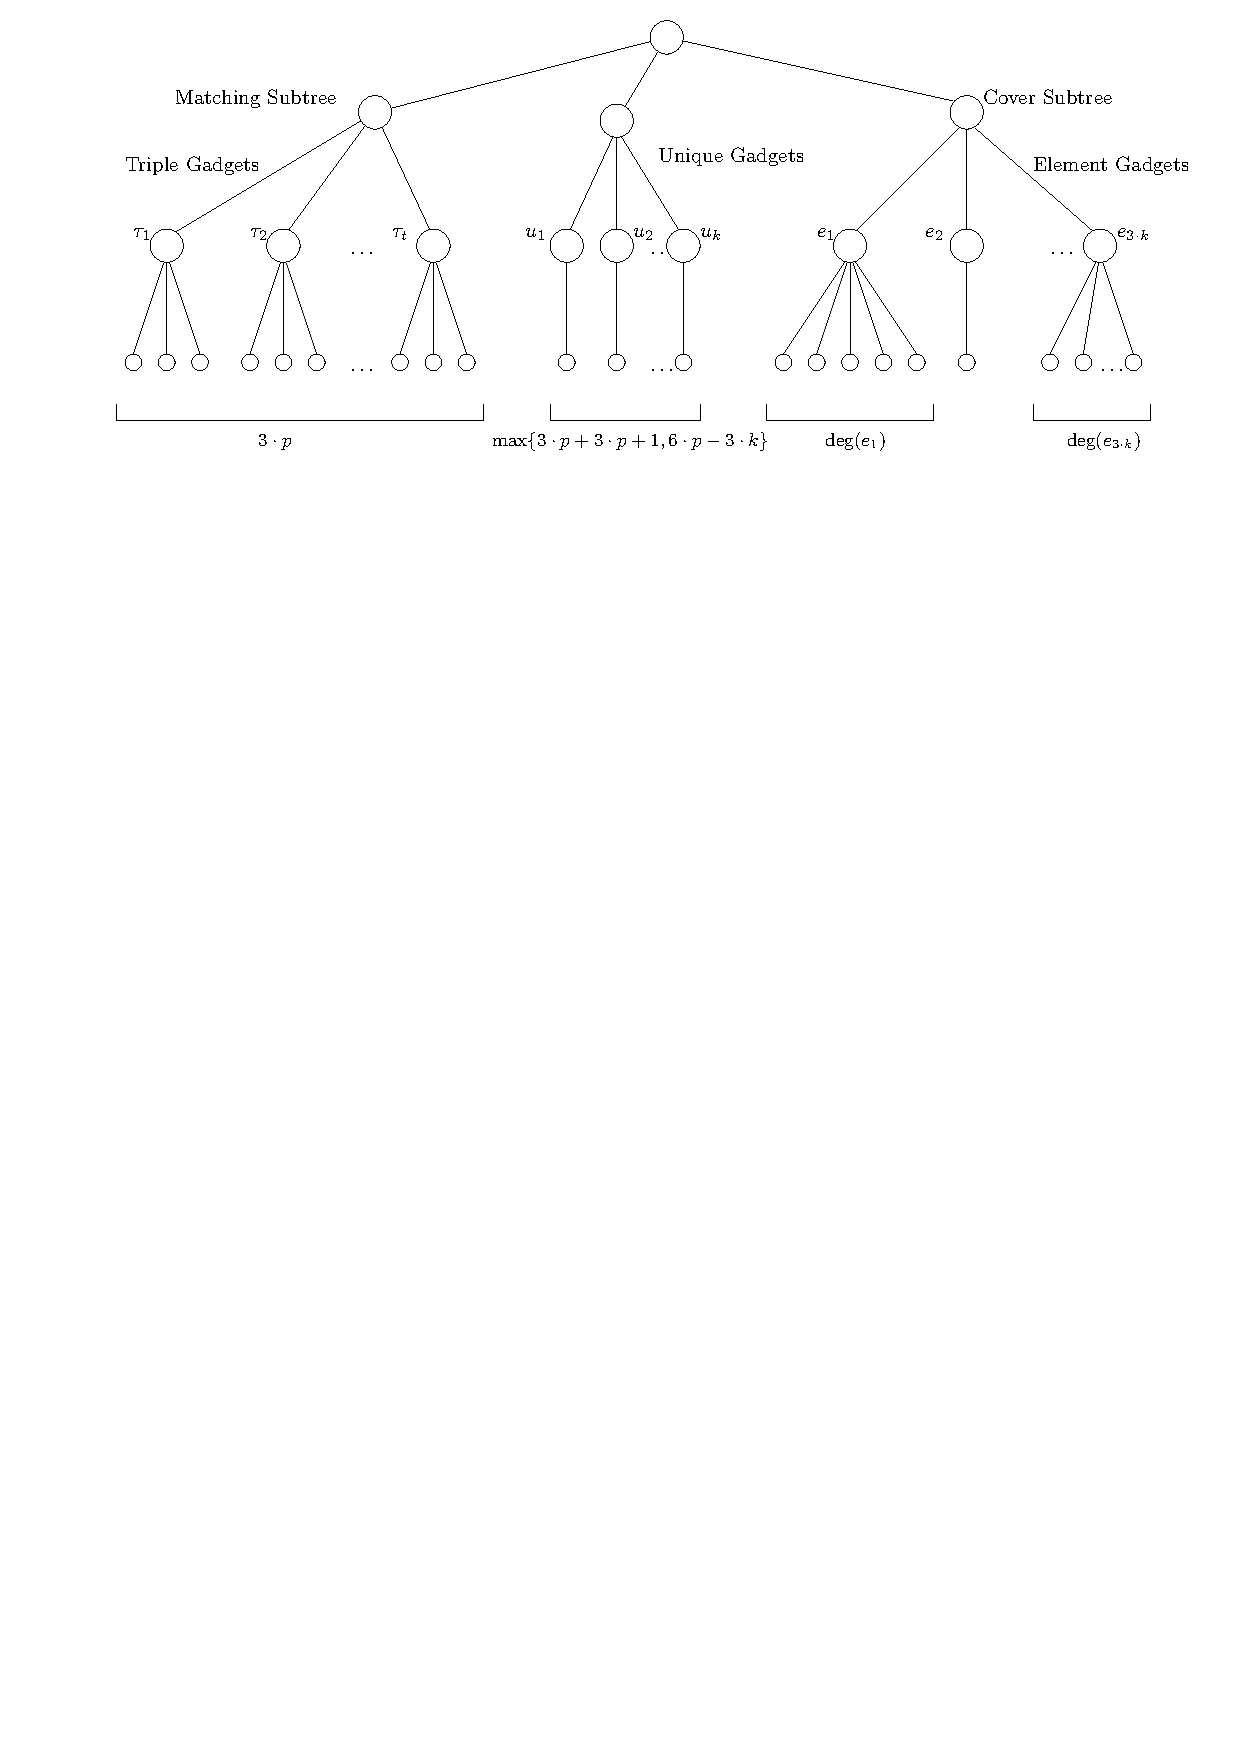
\includegraphics[width=0.99\columnwidth]{figs/static-mapping/overview2}
  \label{fig:red-cc}
  \vspace{-1em}
  \caption{Overview of the substrate network}
  \vspace{-1em}
\end{figure}

\begin{enumerate}
  \item The physical network consists of three subtrees connected to
  the root: the {\MatchSubtree}, the {\CoverSubtree}, and a
  {\UnqSubtree}. In the {\MatchSubtree} we put $t$
  {\TripleGadgets}. The {\CoverSubtree} consist of~$k$ element gadgets.
  \item The {\UnqSubtree} consist of~$|U|$ leaves, and two middle nodes:
  a lower and an upper middle node. Note that this is different from $\RS(2)+\FP+\MA(4)$ NP-completeness proof, where {\UnqSubtree} was placed in the {\MatchSubtree}.
  \item \TripleGadget: For each triple, we create a subtree
  consisisting of four vertices: three leaves and one triple root.  We
  attach the root of the triple to the root of the matching subtree.
  \item \ElGadget: For each element~$e \in X\cup Y\cup Z$, we
  construct a subtree consisting of the root of the element (attached
  to the root of the cover subtree), and~$\deg(e)$ leaves.
\end{enumerate}

\emph{Chunk placement.}
The chunks are placed as follows:
\begin{enumerate}
  \item \emph{Chunks in the Matching Subtree:} In {\TripleGadget} of triple $\tau$ we put
  three replicas:
 ~$ch_1(e_X(\tau), \tau), ch_1(e_Y(\tau), \tau), ch_1(e_Z(\tau), \tau)$, one per each leaf.
  \item \emph{Chunks in the Unique Subtree:} We place replicas
 ~$U$ at the leaves of \UnqGadgets.
 \item \emph{Chunks in Element Gadgets:} Consider the \ElGadget{} for the element $e \in X\cup Y\cup Z$.
 We place two types of replicas in the leaves of the gadget.
 We put replicas $ch_2(\tau, e)$ for each $\tau \in T_e$.
 In total, we place $\deg(e)$ replicas, one per each leaf of the gadget.
\end{enumerate}

\emph{Bandwidth constraints.} We use bandwidth constraints of the form
$\Band(k) := k\cdot(\numNodes - k)$, where $\Vms$ is the total number of nodes to be spawned in the instance. Namely, we set the bandwidth
constraints of an uplink of an {\ElGadget} for each element~$e$ to 
$\Band(\deg(e)-1)$, the bandwidth of an uplink of a~$\MatchSubtree$ to 
$\Band(n)$, and an uplink of a~$\CoverSubtree$ to 
$\Band(\sum_e (\deg(e)-1)$.
Note that out of $\deg(e)$ leaves of \ElGadget{} for element $e$, we allow to spawn $\deg(e)-1$ nodes.

\emph{The threshold value and other properties of the instance.} We set the
cost threshold for any solution to the following value:

\begin{footnotesize}
\begin{align*}
  \Thr  & = 2\cdot \binom{3}{2}\cdot k & \mbox{(over 2 hops in the \MatchSubtree{})}\\
        & + 4 \cdot \binom{3\cdot k}{2} & \mbox{(over 4 hops in the \MatchSubtree{})}\\
        & + 4 \cdot \binom{u}{2} & \mbox{(over 4 hops in the \UnqGadgets{})}\\
        & + \sum_e 2\cdot\binom{\deg(e)-1}{2} & \mbox{(over 2 hops in the \CoverSubtree{})}\\
        & + 4\cdot \binom{\sum_e(\deg(e)-1)}{2} & \mbox{(over 4 hops in the \CoverSubtree{})}\\
        & + 6\cdot\binom{\Vms}{2} & \mbox{(over 6 hops)}
\end{align*}
\end{footnotesize}

where $\Vms$ is the total number of nodes to be spawned in the instance, and $u = |U|$.
  We
set~$\CostTrans$, the cost of chunk transportation to $\Thr+1$ (so that no chunk transportation happens in any feasible solution), 
$\CostCom = 1$, and we host only one node per machine. We set the
number of machines to spawn to:
$\numNodes := 3\cdot k + \sum_e (\deg(e)-1) + |U|$.
\\

\noindent \textbf{Properties of the substrate network.}
\begin{lemma}
  Assume we have a~$\RS(2)+\FP+\CC+\BW$ instance~$I$ with a subtree
 ~$T'$ with~$l$ leaves and the bandwidth capacity on uplink of~$T'$ is
 ~$\Band(k)$. Assume that no chunk transportation is allowed
  ($\CostTrans = \infty$, so every node must be collocated with the
  chunk it processes in every feasible solution), and~$\CostCom = 1$.
  Then in any feasible solution the number $s$ of nodes spawned in~$T$ satisfies~$s \leq k \vee \Vms-s\leq k$, and~$s \leq l$.
  \label{lem:bandwidth1}
\end{lemma}

\begin{proof}
It holds that ~$s\leq l$ as we cannot spawn more nodes than leaves.
  The bandwidth allocation on the uplink of~$T'$ is
 ~$uplink(s,T) := s\cdot (\Vms - s)$, as no chunk transportation
  is allowed ($\CostTrans = \infty$), and every node in~$T$ has to
  communicate over~$T'$'s uplink with nodes spawned outside of
 ~$T'$. Therefore, in every feasible solution we have:
 ~$uplink(s, T') \leq \Band(k)$.  Let's define the remaining bandwidth
  on the uplink of $T'$~$\remainBw(s) := \Band(k)-uplink(s, T') = s^2 - s\cdot \Vms -
  k^2+k\cdot \Vms~$.
  Every feasible solution fulfills~$\remainBw(s) \geq 0$, which is true for
 ~$s \leq k \vee \Vms-s\leq k$ (follows from the properties of the
  quadratic function).
\end{proof}


Next, we show how to precisely control the number of nodes in the
constructed subtree.

\begin{obs}
  In every feasible solution we have exactly~$|U|$ nodes spawned in a
  {\UnqSubtree} (no chunk transportation is allowed, and every chunk
  type must be processed).
  \label{obs:unq-full}
\end{obs}


\begin{lemma}
  The following properties holds in $S_{\VCEMB}$:
  \begin{enumerate}
    \item The number of nodes spawned in a {\MatchSubtree} is
   ~$3\cdot k$.
    \item The number of nodes spawned in a {\CoverSubtree} is
   ~$\sum_e(\deg(e)-1)$
  \end{enumerate}

  \label{lem:bandwidth2}
\end{lemma}

\begin{proof}
  From Observation~\ref{obs:unq-full} we know that we have~$|U|$ nodes
  in the {\UnqSubtree}. Let's refer to the number of nodes spawned in
  a {\MatchSubtree} by~$M$, and to the number of nodes spawned in
  {\CoverSubtree} by~$C$. By applying Lemma~\ref{lem:bandwidth1} to
  {\MatchSubtree}, we know that: $ M \leq 3\cdot k \vee M \geq \Vms - 3\cdot k$.
  We observe that~$\Vms - 3\cdot k$ is greater than the number of
  leaves in a {\MatchSubtree}.  By applying Lemma~\ref{lem:bandwidth1}
  to the {\CoverSubtree} we know that:~$ C \leq \sum_e(\deg(e)-1) \vee C$ $\geq \Vms - \sum_e(\deg(e)-1)$.
  We observe that~$\Vms - \sum_e(\deg(e)-1)$ is greater than the number
  of leaves in the {\CoverSubtree}.
  We also know that~$\Vms = |U| + C + M$. Therefore, by the pigeon-hole principle
 ~$C = \sum_e(\deg(e)-1)$ and~$M = 3\cdot k$.
\end{proof}


\begin{lemma}
  In $S_{\VCEMB}$ the number of nodes spawned in Element Gadget of
  element~$e$ is~$\deg(e)-1$.
  \label{lem:bandwidth3}
\end{lemma}

\begin{proof}
  Let's call the number of nodes spawned in the Element Gadget of
  element~$e$ the $x_e$.  From Lemma~\ref{lem:bandwidth1}, we know that
 ~$x_e \leq \deg(e) - 1 \vee x_e \geq \Vms - \deg(e) + 1$. We observe
  that~$\Vms - \deg(e) + 1$ is greater than the number of leaves of the
  gadget, which is~$\deg(e)$.  From Lemma~\ref{lem:bandwidth2}, we know
  that the number of nodes spawned in the entire {\CoverSubtree} is
 ~$\sum_e (\deg(e)-1)$. Therefore, by the pigeon-hole principle, we have
  that~$x_e = \deg(e)-1$.
\end{proof}

From the above lemmas we know the precise number of nodes spawned in
certain parts of the tree. Feasible solutions only differ in 
the choice of the~$\deg(e) - 1$ out of~$\deg(e)$ chunks
in each Element Gadget, and the placement of nodes in the
{\MatchSubtree}.



Similar in spirit to the NP-completeness proof of~$\RS(2)+\MA(4)+\FP$,
we call the {\TripleGadget} active if it contains exactly three nodes. 
Similarly, we call the {\TripleGadget} inactive if it
does not contain spawned nodes, and \emph{partially active} if it
has one or two
spawned nodes.

\begin{lemma}
  In $S_{\VCEMB}$, we have exactly~$k$ active
  {\TripleGadgets}.
  \label{lem:full-or-empty}
\end{lemma}

\begin{proof}
  Since~$I$ is feasible, we know that it has a solution~$\Sol$ of
  cost~$\leq \Thr$.
  By Lemma~\ref{lem:bandwidth2}, we know that there are
  exactly~$3\cdot k$ spawned nodes in the {\MatchSubtree}. Therefore, by
  the pigeon-hole principle, we know that we have at most~$k$
  active {\TripleGadgets}. It remains to show that there
  are no partially active {\TripleGadgets} in the solution of cost
 ~$\leq \Thr$.
  Using Lemma~\ref{lem:bandwidth3}, 
  we conclude that the communication cost of
  nodes in the {\CoverSubtree} is the same for every feasible solution
  (let's name that cost~$P$). We also know that the communication cost
  between nodes in {\CoverSubtree} and {\MatchSubtree} is the same for
  every feasible solution (let's name it~$Q$). Let's call the
  would-be cost of communication in the {\MatchSubtree}, if there were
  exactly~$k$ active gadgets,~$R$.
  The threshold value was chosen so that~$\Thr = P+Q+R$. If we have at least one partially active
  gadget, then the cost of communication in {\MatchSubtree} is greater
  than~$R$, because we increase the number of 4-hop communications by
  at least one per each partially active gadget in comparison to a solution
  where we have exactly~$k$ active gadgets.
\end{proof}

\noindent \textbf{The reduction.}
Using the properties of the substrate network, we perform the reduction in the following way.

\begin{theorem}
 ~$\RS(2)+\FP+\CC+\BW$ is NP-hard.
\end{theorem}

\begin{proof}
  Let's take any instance $I_{\TDPM}$ of~$\TDPM$.
  We show that~$I_{\VCEMB}$ has a solution of cost~$\leq \Thr$ if and only if~$I_{\TDPM} \in \TDPM$ (there exists a perfect 3D matching in $I_{\TDPM}$).


  Let's take an instance~$I$ of~$\TDPM$ and construct an instance~$I'$
  of~$\RS(2)+\FP+\CC+\BW$ in the way described above.  We show that
 ~$I'$ has solution of cost~$\leq \Thr$ if and only if~$I \in \TDPM$
  (there exists a perfect 3D matching).

  ($\Leftarrow$) Let's take any feasible solution~$S_{\TDPM}$ to~$I_{\TDPM}$ and
  produce a solution~$S_{\VCEMB}$ to~$I_{\VCEMB}$ in the way described in the construction section. We show that the cost of~$S_{\VCEMB}$ is
  indeed~$\leq \Thr$.
  For each triple~$t\in T$ in~$S_{\TDPM}$, we put~$3$ nodes at
  leaves of triple gadgets corresponding to those triples.  In each
  element gadget (that corresponds to element~$e$), we put~$\deg(e)-1$
  nodes. In each element gadget there is only one leaf without the
  node placed in it: this node contains the chunk replica that is
  processed in the {\MatchSubtree}.
  It is easy to see that~$S_{\VCEMB}$ has cost exactly~$\Thr$ and no
  bandwidth constraint is violated. Each chunk type is processed.

  ($\Rightarrow$) Let's take any feasible solution~$S_{\VCEMB}$ to~$I_{\VCEMB}$ and
  produce a solution~$S_{\TDPM}$ to~$I_{\TDPM}$ by taking triples that correspond
  to active triple gadgets. Using Lemma~\ref{lem:full-or-empty}, we
  conclude that there are exactly~$k$ active triple gadgets. By
  feasibility of~$S_{\TDPM}$, we know that each chunk type is
  processed. From Lemma~\ref{lem:bandwidth3}, we know that out
  of~$\deg(e)$ chunk types that correspond to~$e\in X\cup Y\cup Z$,
  exactly one is processed in the {\MatchSubtree}, hence each
  element of~$X\cup Y\cup Z$ is matched.
\end{proof}


%%%%%%%%%%%%%%%%%%%%%%%%%%%%%%%%%%%%%
\section{Summary}\label{sec:conclusion}

In this chapter we have shown that despite the
multiple dimensions of flexibility in terms of chunk assignment and node placement, 
and despite the large scale of modern datacenters, 
many problems can be solved efficiently. However, we have also
shown that several embedding problems are NP-hard already in two-
and three-level trees---a practically relevant result given today's datacenter topologies~\cite{fattree}.


%\begin{table}
%\tiny
%\bgroup
%\def\arraystretch{1.5}
%\begin{small}
%\begin{tabular}{|l|l|p{6.5cm}|}
%\hline
%\multirow{3}{*}{NP-hard} & 5 combinations & \mbox{$\RS+\MA+\FP+\CC+\BW$}\\
%\cline{2-3}
% & 4 combinations &  \mbox{$\RS+\MA+\FP+\CC$}; \mbox{$\RS+\MA+\FP+\BW$};
%\mbox{$\RS+\FP+\CC+\BW$} \\ \cline{2-3}
% & 3 combinations &\mbox{$\RS+\MA+\FP$};~\mbox{$\RS+\FP+\CC$} \\
% \hline
% \hline
%\multirow{3}{*}{Flow} & 4 combinations & \mbox{$\RS+\MA+\CC+\BW$} \\ \cline{2-3}
% & 3 combinations & \mbox{$\RS+\CC+\BW$}; \mbox{$\RS+\MA+\BW$}    \\ \cline{2-3}
% & 2 combinations &$\RS+\BW$ \\
% \hline
% \hline
%\multirow{3}{*}{DP} & 4 combinations & \mbox{$\MA+\FP+\CC+\BW$} \\ \cline{2-3}
% & 3 combinations &   \mbox{$\MA+\FP+\CC$};
%\mbox{$\MA+\FP+\BW$}; \mbox{$\FP+\CC+\BW$} \\ \cline{2-3}
% & 2 combinations & \mbox{$\MA+\FP$};~\mbox{$\FP+\CC$}; \\
% \hline
% \hline
%\multirow{3}{*}{Matching} &3 combinations&
%\mbox{$\RS+\MA+\CC$};~\mbox{$\MA+\CC+\BW$}  \\
%\cline{2-3}
% & 2 combinations & \mbox{$\RS+\MA$};
%\mbox{$\RS+\CC$}; \mbox{$\MA+\CC$};
%\mbox{$\MA+\BW$}; \mbox{$\CC+\BW$} \\ \cline{2-3}
%& 1 combinations & \mbox{$\RS$}; \mbox{$\MA$};
%\mbox{$\CC$}; \mbox{$\BW$}\\
% \hline
% \hline
% \multirow{3}{*}{0 Cost} & 3 combinations & \mbox{$\RS+\FP+\BW$}\\
%\cline{2-3}
% & 2 combinations & \mbox{$\RS+\FP$}; \mbox{$\FP+\BW$}\\ \cline{2-3}
% & 1 combinations & \mbox{$\FP$}\\
% \hline
%\end{tabular}
%\end{small}
%\caption{
%Fastest algorithms for different respective problem variants.
%}
%\vspace{-2em}
%\label{tab:summary}
%\egroup
%\end{table}

\begin{figure}[t]
\centering
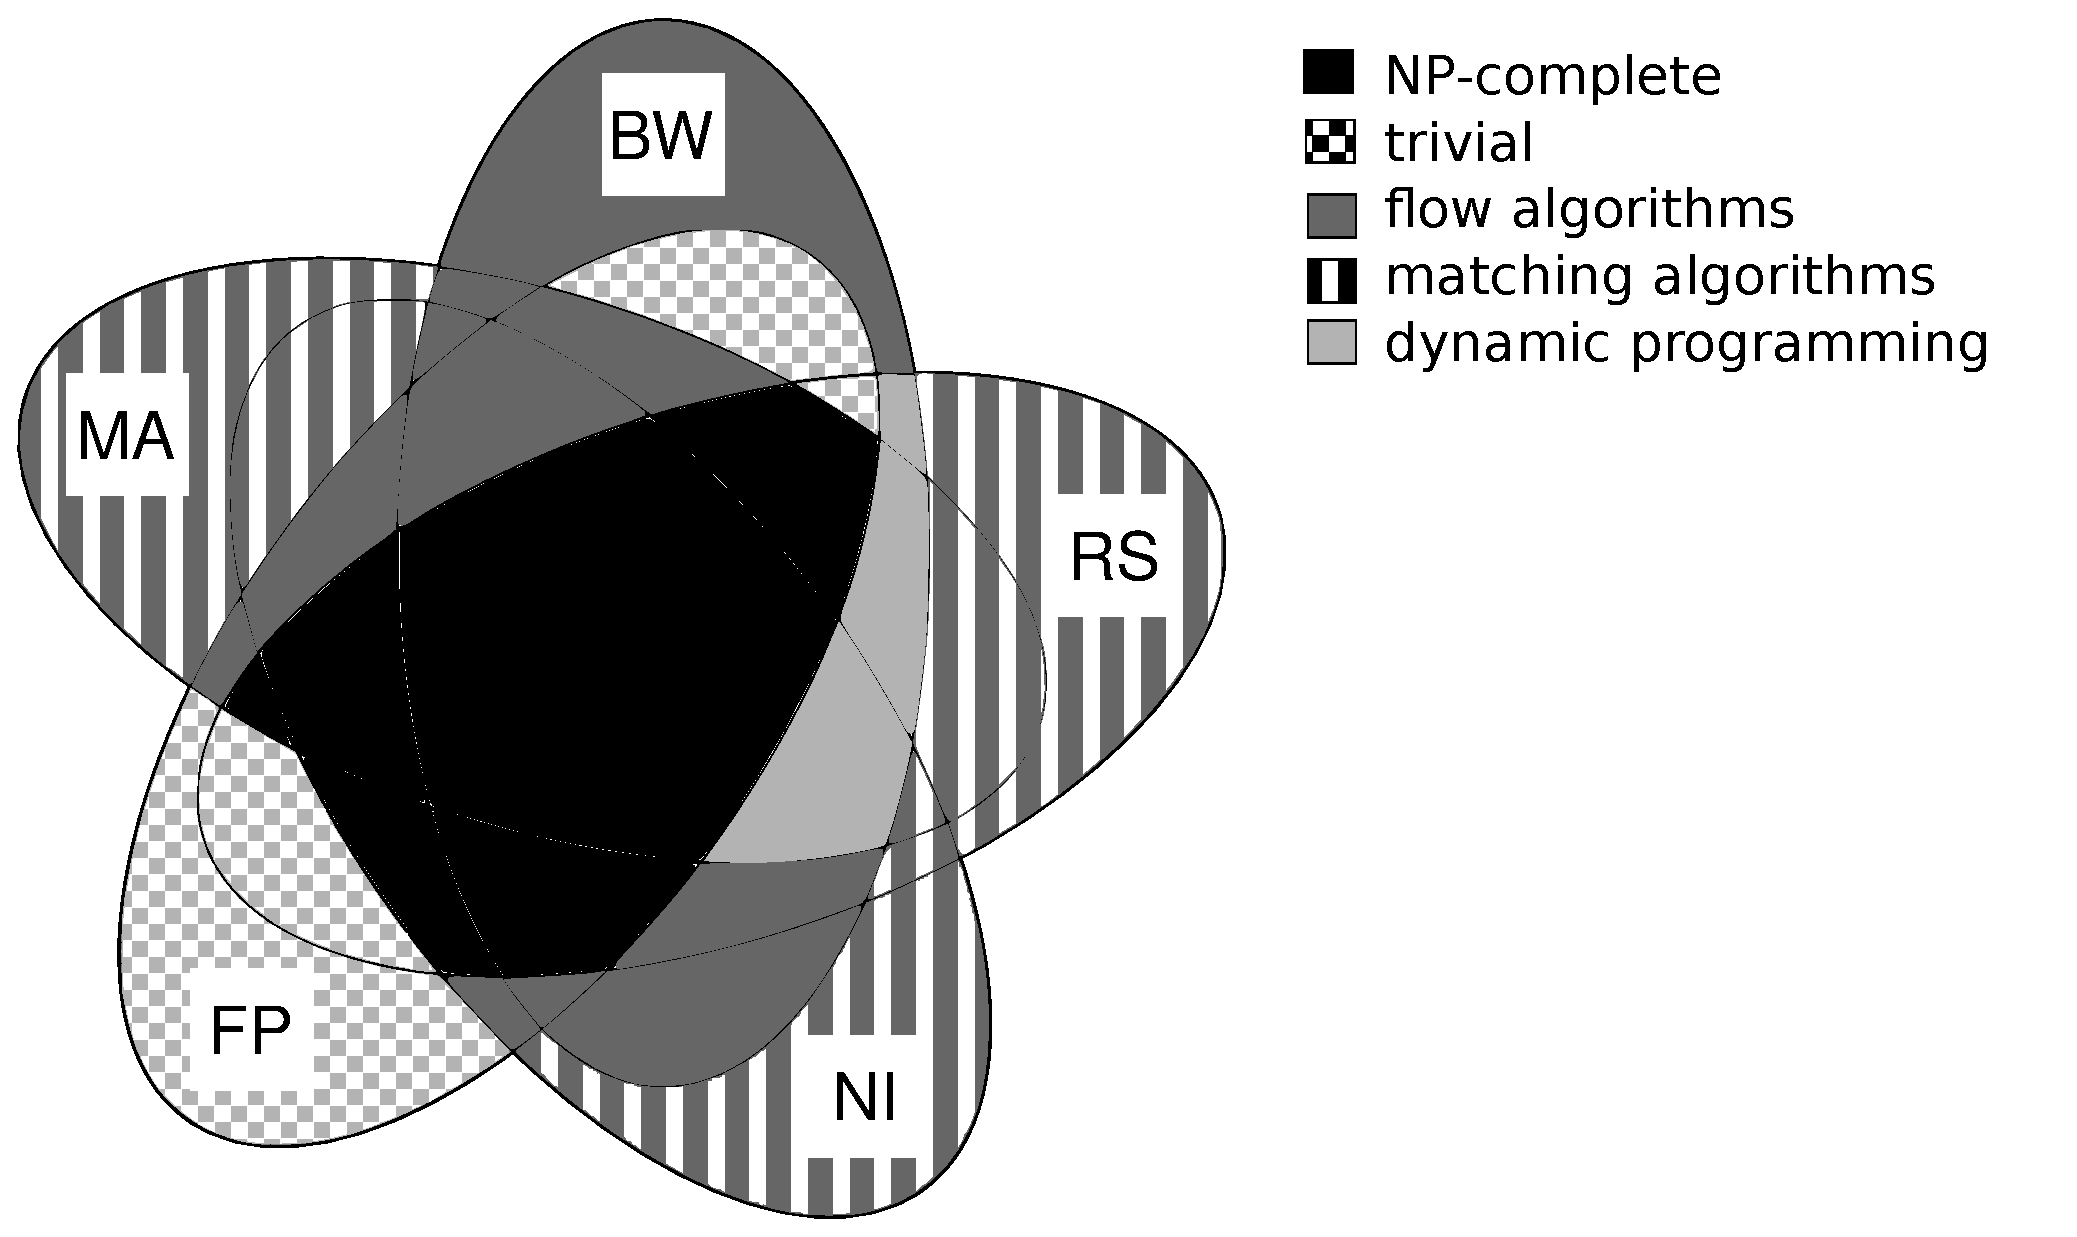
\includegraphics[width=0.69\columnwidth]{figs/static-mapping/venn_full2.pdf}
\caption{Fastest algorithms for different respective problem variants. Variants depicted by solid black are NP-hard, and variants depicted by checked filling are trivially solvable. For the remainder of variants we provide the fastest algorithm determined by the key.}
\vspace{-1em}
\label{fig:venn_full}
\end{figure}




Our results are summarized in
Figure~\ref{fig:venn_full}.
One interesting takeaway from this figure regards
the question which properties render the problem
NP-hard. For instance, we see that,~$\BW$
does not influence the hardness of any problem variant,
while~$\RS$ is crucial for NP-hardness.
$\MA$ only affects hardness if combined with~$\RS$.
$\CC$ is trivial without~$\FP$, and~$\FP$ requires
more sophisticated algorithms when combined with~$\CC$ or~$\MA$;
in combination with~$\RS$ and~$\MA$ or~$\CC$,~$\FP$ renders the
problem NP-hard.
